\documentclass[../Head/Main.tex]{subfiles}
\begin{document}
\section{Vision}
\label{sec:vision}
In this section a complete walk through of the thoughts, methods and results of the different vision algorithms, that has been implemented are analysed and tested to locate a breach. The methods that will be analysed in this section include: Fourier Transformation to find the rectangular pattern in a fence structure, image segmentation using U-Net deep-learning method, a canny edge detection as well as a convolutional approach to segment the fence from the background and lastly a Convolutional Neural Network.    

\subsection{Analysing the different sensor options}
\label{subsec:analyse_the_approches}

Using a LiDAR could prove to be a powerful tool and a very interesting approach to follow. However, with the given drone, which has a current weight of 2500g, see Appendix \ref{app:drone_specifications}, and a maximum takeoff weight (MTOW) of 3200g, this lead to a total added weight from external sensors of: $3200g - 2500g = 700g$. For the lower end price of LiDAR's it is not uncommon that it weights over 1kg. Which is undesirable. It is possible to find a LiDAR below 700g. However, they come with a cost which is not suitable for this project. Thus, no further exploration of the use of LiDAR will be conducted. \\
A cheap and viable solution would be to use a Intel Realsense D435 Depth Camera. This will give access to multiple sensor within this one device, as well as a cheap cost of below 2500 DKK. It will grand access to a mono-RGB camera, depth sensor and even stereo cameras if needed \cite{Intel_RS_price}.

\subsubsection{Depth Camera Analysis}
\label{subsubsec:depth_camera_analysis}
Depth camera is a powerful tool which provides depth and distance information for the objects in the images. The basic principle of depth camera is either projecting IR or structured light to get depth information or using closely placed cameras for capturing and comparing images (Stereo setup). Depth images are relatively easy to process, because of the depth information associated with the pixels. We tested the Intel RealSense D435 Depth Camera which uses active IR stereo to generate depth images.

\begin{figure}[H]
    \centering
    \includegraphics[width=0.75\textwidth]{../Figures/active_IR.png}
    \caption{Depth Sensor Configurations}
    \label{fig:depth_data}
\end{figure}

Initially the idea of using the depth camera was to generate a point cloud only consisting of points between 1 and 4 meters away. These point would then be used to reconstruct the grid structure of the fence and a breach could be detected. In theory this would work, but as we discovered, when dealing with actual data from the sensor, the data was unusable for this approach, see \autoref{fig:depth_data}.

\begin{figure}[H]
    \centering
    \includegraphics[width=0.75\textwidth]{../Figures/depth_img.png}
    \caption{Real life data from depth sensor}
    \label{fig:depth_data}
\end{figure}

This data is not usable for our approach, however a new hypothesis was made, that using some mean value distance of multiple points within the center of the image could perhaps be utilised to maintain a certain distance from the fence at all times. 

\subsection{Segmentation of The Image}
\label{subsec:seg_image}
This section will go through and analyse four different approaches to segment an image. During segmentation the goal is to remove as much as the background as possible, without compromising the fence structure. This is required to leave as little as possible to interfere with the screening algorithm. See \autoref{subsec:screening_for_breaches}. 
\par 
This algorithm will systematic go through the grid structure of the fence, locating intersections and detecting obstructions in this structure to verify a breach and its size.

\subsubsection{Fourier Transformation}
\label{seg:fouier_transformation}
A way to separate the background from the fence was to use the Fourier Transformation which can decompose an image into its sine and cosine components. The output will be given in the frequency domain with the input given in the spatial domain. In this frequency domain each point represents a given frequency in the spatial image domain.

The two-dimensional Discrete Fourier Transformation (DFT) and its inverse is given in Equation \ref{eq:DFT_and_inverse} respectively. 

\begin{equation}
    F(k,l) = \sum_{i=0}^{N-1} \sum_{j=0}^{N-1} f(i,j) e^{\tau 2 \pi \left( \frac{ki}{N} + \frac{lj}{N}\right)} \qquad  
        f(a,b) = \frac{1}{N^2} \sum_{k=0}^{N-1} \sum_{l=0}^{N-1} F(k,l) e^{\tau 2 \pi \left( \frac{ka}{N} + \frac{lb}{N} \right)}
    \label{eq:DFT_and_inverse}
\end{equation}

Here the $f(a,b)$ is the image in the spatial domain with the exponential as the basis function that corresponds to every point $F(k,l)$ in the Fourier transform. Hence the value for each point $F(k,l)$ is obtained by a multiplication of the spatial image with the corresponding base function and summing the results. The $F(0,0)$ is the DC-component (average brightness) and $F(N-1,N-1)$ is the highest frequency. The term $\frac{1}{N^2}$ is used as a normalisation term. The Fourier Transform is separable therefore it can be rewritten as seen in Equation \ref{eq:DFT_separable}. 

\begin{equation}
    f(a,b) = \frac{1}{N} \sum_{b=0}^{N-1} P(k,b) e^{\tau 2 \pi \frac{lb}{N}} \qquad
       P(k,b) = \frac{1}{N} \sum_{a=0}^{N-1} f(a,b) e^{\tau 2 \pi \frac{ka}{N}}
    \label{eq:DFT_separable}
\end{equation}

Calculating a two-dimensional Fourier Transformation can be done using a series of two one-dimensional calculations. This decreases the amount of required computations, yielding a $O(N^2)$ computational time. To improve further a Fast Fourier Transformation (FFT) could be used, which reduces the time complexity to $O(N log_2 N)$. This was one of the main reasons for choosing the Fourier Transformation to segment the fence from the background. Since this enables the calculations to be done very fast and utilises the possibility of detecting breaches closer to real-time.\cite{FFT}    
\par

\textbf{Analysis:}\\
The performance evaluation of the FFT will be based on images in different configurations. This is done to stress test the algorithm, in order to find its limitations. The code used for this algorithm was heavily inspired by a script given from Henrik Skov Midtiby (\textit{hemi@mmmi.sdu.dk}) which involves FFT in Python and OpenCV. The procedure will follow the approach described in Section \ref{seg:fouier_transformation}. Given the image in \autoref{fig:image_without_breach}, the Fourier spectrum was found and visualised in \autoref{fig:fourier_mask_without_breach}. Here the structure of the fence is nicely highlighted as seen in the frequency spectrum of the FFT. The mask is now multiplied with the input image and the results can be seen in \autoref{fig:fouier_original_image}.

\begin{figure}[H]
    \centering
    \begin{subfigure}{.48\textwidth}
        \centering
        \includegraphics[width=\textwidth]{../Figures/fourier_transformation/fence_clean.png}
        \caption{Input image of fence without breaches.}
        \label{fig:image_without_breach}
    \end{subfigure}
    \hfill
    \begin{subfigure}{.48\textwidth}
        \centering
        \includegraphics[width=\textwidth]{../Figures/fourier_transformation/fence_mask.png}
        \caption{Fourier spectrum of input image (mask).}
        \label{fig:fourier_mask_without_breach}
    \end{subfigure}
    \label{fig:input_and_fouier}
            \begin{subfigure}{.48\textwidth}
        \centering
        \includegraphics[width=\textwidth]{../Figures/fourier_transformation/fence_clean_20_low_pass_filtered.png}
        \caption{Multiplication of mask and input image.}
        \label{fig:fouier_original_image}
    \end{subfigure}
    \caption{Illustration of the working of the Fourier transformation resulting in a background subtraction of the image in Figure \ref{fig:fouier_original_image}}
\end{figure}
\vspace{-15pt}

The results is a segmented image where only the structure of the fence is visible. It may the noticed that this image is underexposed which results in a fine separation of the foreground (fence) and background (forest). This image is taken under ideal conditions in regard to optimising the performance of the FFT. 

\begin{figure}[H]
    \centering
    \begin{subfigure}{.48\textwidth}
        \centering
        \includegraphics[width=\textwidth]{../Figures/fourier_transformation/fence_breach.png}
        \caption{Input image of fence with breach.}
        \label{fig:input_image_breach}
    \end{subfigure}
    \hfill
    \begin{subfigure}{.48\textwidth}
        \centering
        \includegraphics[width=\textwidth]{../Figures/fourier_transformation/fence_breach_mask.png}
        \caption{Fourier spectrum of input image (mask).}
        \label{fig:fouier_detected_with_breaches}
    \end{subfigure}
    \hfill
    \begin{subfigure}{.48\textwidth}
        \centering
        \includegraphics[width=\textwidth]{../Figures/fourier_transformation/fence_breach_20_low_pass_filtered.png}
        \caption{Multiplication of Mask and input image with breaches}
        \label{fig:fourier_mask_with_breach}
    \end{subfigure}    
    \caption{Input image with breaches and the resulting background subtracted image suing Fourier transformation}
\end{figure}

Now giving an input image with customised breaches, the Fourier spectrum can be seen in Figure \ref{fig:fourier_mask_with_breach}. Applying this mask on the input image the resulting segmentation can be seen in Figure \ref{fig:fouier_detected_with_breaches}. From this result it is possible to detect the breaches. The algorithm made to conquer this problem can be seen in Section \ref{subsec:screening_for_breaches}.   

\begin{figure}[H]
    \centering
    \begin{subfigure}{.32\textwidth}
        \centering
        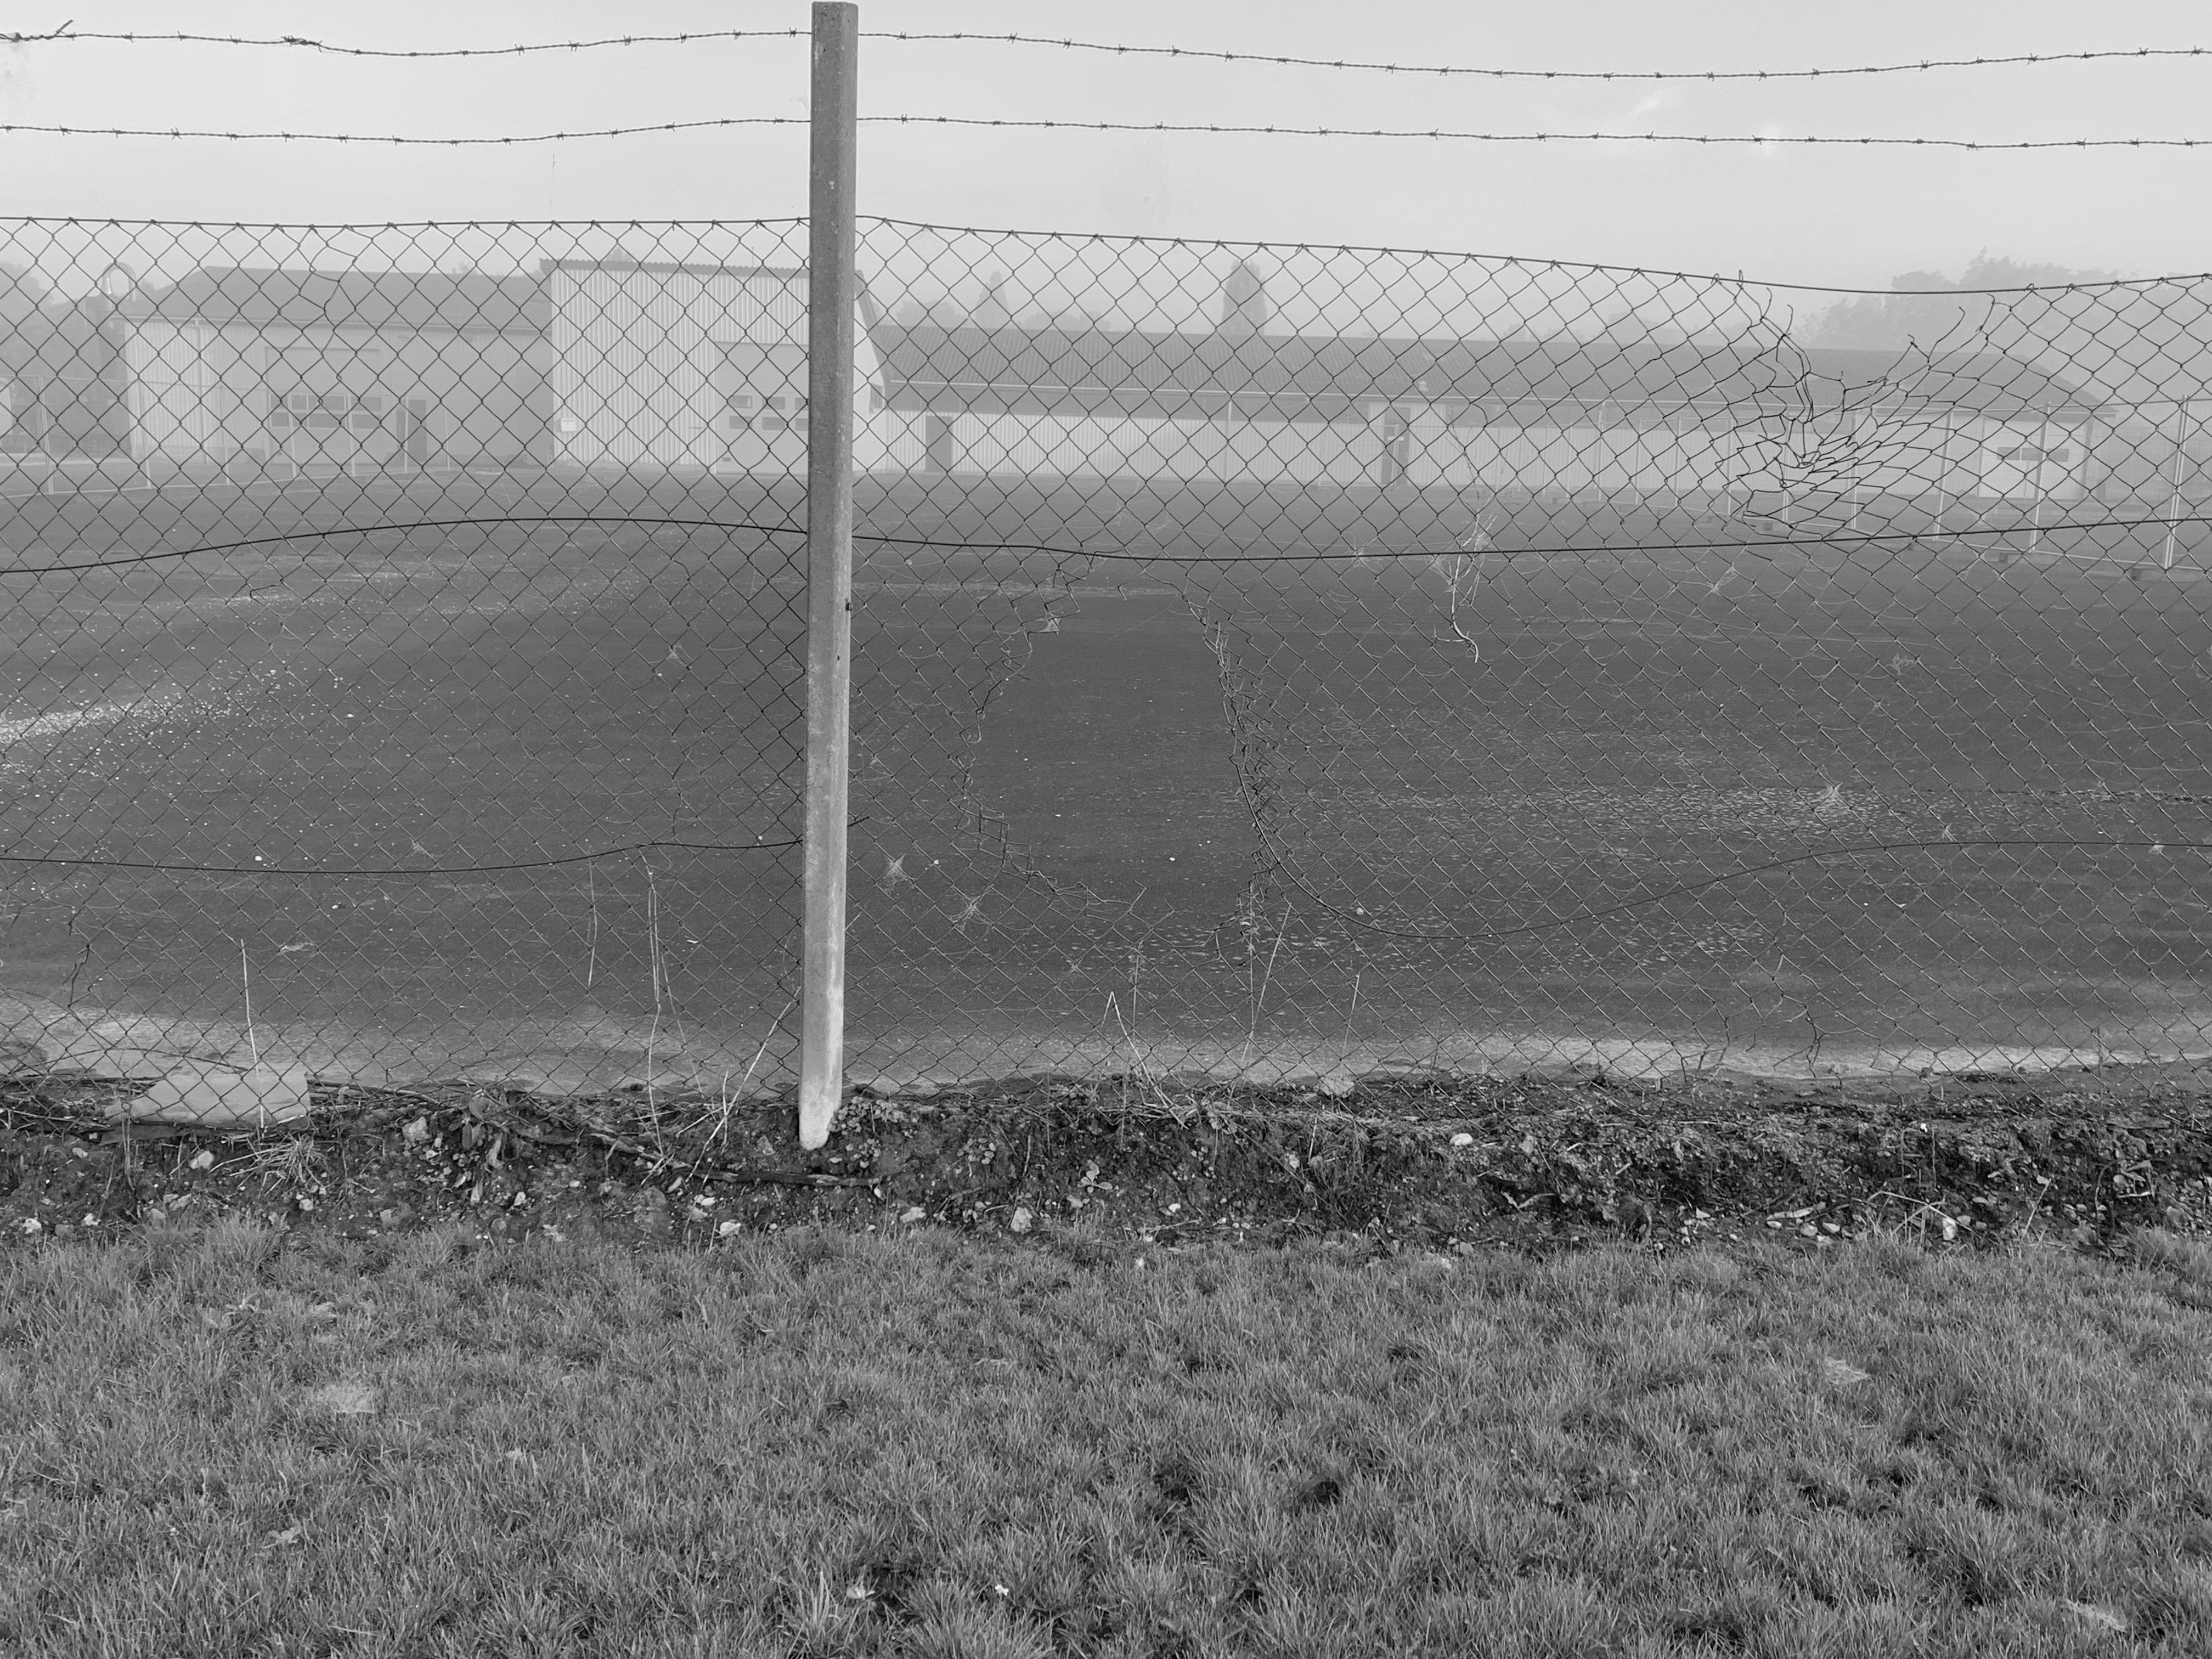
\includegraphics[width=\textwidth]{../Figures/fourier_transformation/00_input_image_notworking.png}
        \caption{Input image of fence}
        \label{fig:input_image_breach_notworking}
    \end{subfigure}
    \hfill
    \begin{subfigure}{.32\textwidth}
        \centering
        \includegraphics[width=\textwidth]{../Figures/fourier_transformation/07_shifted_fft_peak_mask_notworkning.png}
        \caption{Fourier spectrum (mask)}
        \label{fig:fouier_mask_with_breaches_notworking}
    \end{subfigure}
    \hfill
    \begin{subfigure}{.32\textwidth}
        \centering
        \includegraphics[width=\textwidth]{../Figures/fourier_transformation/20_low_pass_filtered_image_notworking.png}
        \caption{Segmented image}
        \label{fig:fourier_detected_with_breaches_notworking}
    \end{subfigure}    
    \caption{Input image and the resulting background subtracted image using Fourier transformation}
\end{figure}

Because the FFT takes into account certain patterns in the image, it is highly sensitive to variations in light, background and other structures which shows some kind of symmetry. Especially if light is projected on structures in the image which is of no interest. Such an image can be seen in Figure \ref{fig:input_image_breach_notworking}. Here the fence is hard to detect with a gray background. Moreover, the light is not projected on the fence the same way as in Figure \ref{fig:image_without_breach}. This make the problem considerably more challenging. This Fourier spectrum can be seen in Figure \ref{fig:fouier_mask_with_breaches_notworking}. One may notice that the Fourier spectrum includes a lot more frequencies then the ones got in Figure \ref{fig:fourier_mask_with_breach}. As it can be seen in Figure \ref{fig:fourier_detected_with_breaches_notworking}, the background is not properly removed from the input image yielding a very bad segmentation.

Ways to deal with this problem could be to project a light source on the drone reflecting upon the fence. This could make a better separation of the fence from the background. Furthermore, the mask in the Fourier spectrum could be multiplied with a user defined mask excluding the frequencies which have no interest. A visualisation of these improvements can be seen in Figure \ref{fig:fourier_improments}. 

\begin{figure}[H]
    \centering
    \begin{subfigure}{.32\textwidth}
        \centering
        \includegraphics[width=\textwidth]{../Figures/fourier_transformation/dark_img1.jpg}
        \caption{Light projected on the fence}
        \label{fig:image_light_projected}
    \end{subfigure}
    \hfill
    \begin{subfigure}{.32\textwidth}
        \centering
        \includegraphics[width=\textwidth]{../Figures/userdefinedmask.png}
        \caption{User defined mask}
        \label{fig:user_defined_mask}
    \end{subfigure}
    \hfill
    \begin{subfigure}{.32\textwidth}
        \centering
        \includegraphics[width=\textwidth]{../Figures/fouriermultipledbymask.png}
        \caption{Resulting Fourier spectrum}
        \label{fig:fourier_spectrum_multiplied_with_mask}
    \end{subfigure}
    \caption{Input image and the resulting background subtracted image using Fourier transformation}
    \label{fig:fourier_improments}
\end{figure}

Unfortunately, these improvements did not result in a general improvement of the segmentation of the image. The spectrum in the FFT still has to be tuned to fit the given conditions from where the image is taken. This is a considerable drawback of using this algorithm for segmentation. 
\clearpage

\subsubsection{Segmentation using U-Net}
\label{seg:deep_learning_segmentaion}
Another approach for using neural networks, is the fence segmentation using neural networks such as U-Net and then performing the breach detection using the fence re-construction methods discussed in the previous sections. U-Net configuration is particularly good at segmenting images. A typical U-Net used for image segmentation is shown in \autoref{fig:unet_arch}. 

\begin{figure}[H]
    \centering
    \includegraphics[width=0.72\textwidth]{../Figures/unet_arch.png}
    \caption{U-Net Architecture \cite{UNET_fig}}
    \label{fig:unet_arch}
\end{figure}

For each pixel in the input image the U-Net outputs a binary pixel classifying it as either background or foreground. This configuration, if properly trained, could provide a very strong segmentation tool. However, to train the U-Net hundreds of different fence images where needed with specified ground truth or mask of the image. This data was not readily available in our case. However, using generated artificial data sets, some level of performance from the U-Net approach  could be achieved.
\par
An example of the U-Net input image and ground truth is shown in Figure \autoref{fig:unet_input}.

\begin{figure}[H]
    \centering
    \begin{subfigure}{0.49\textwidth}
        \centering
        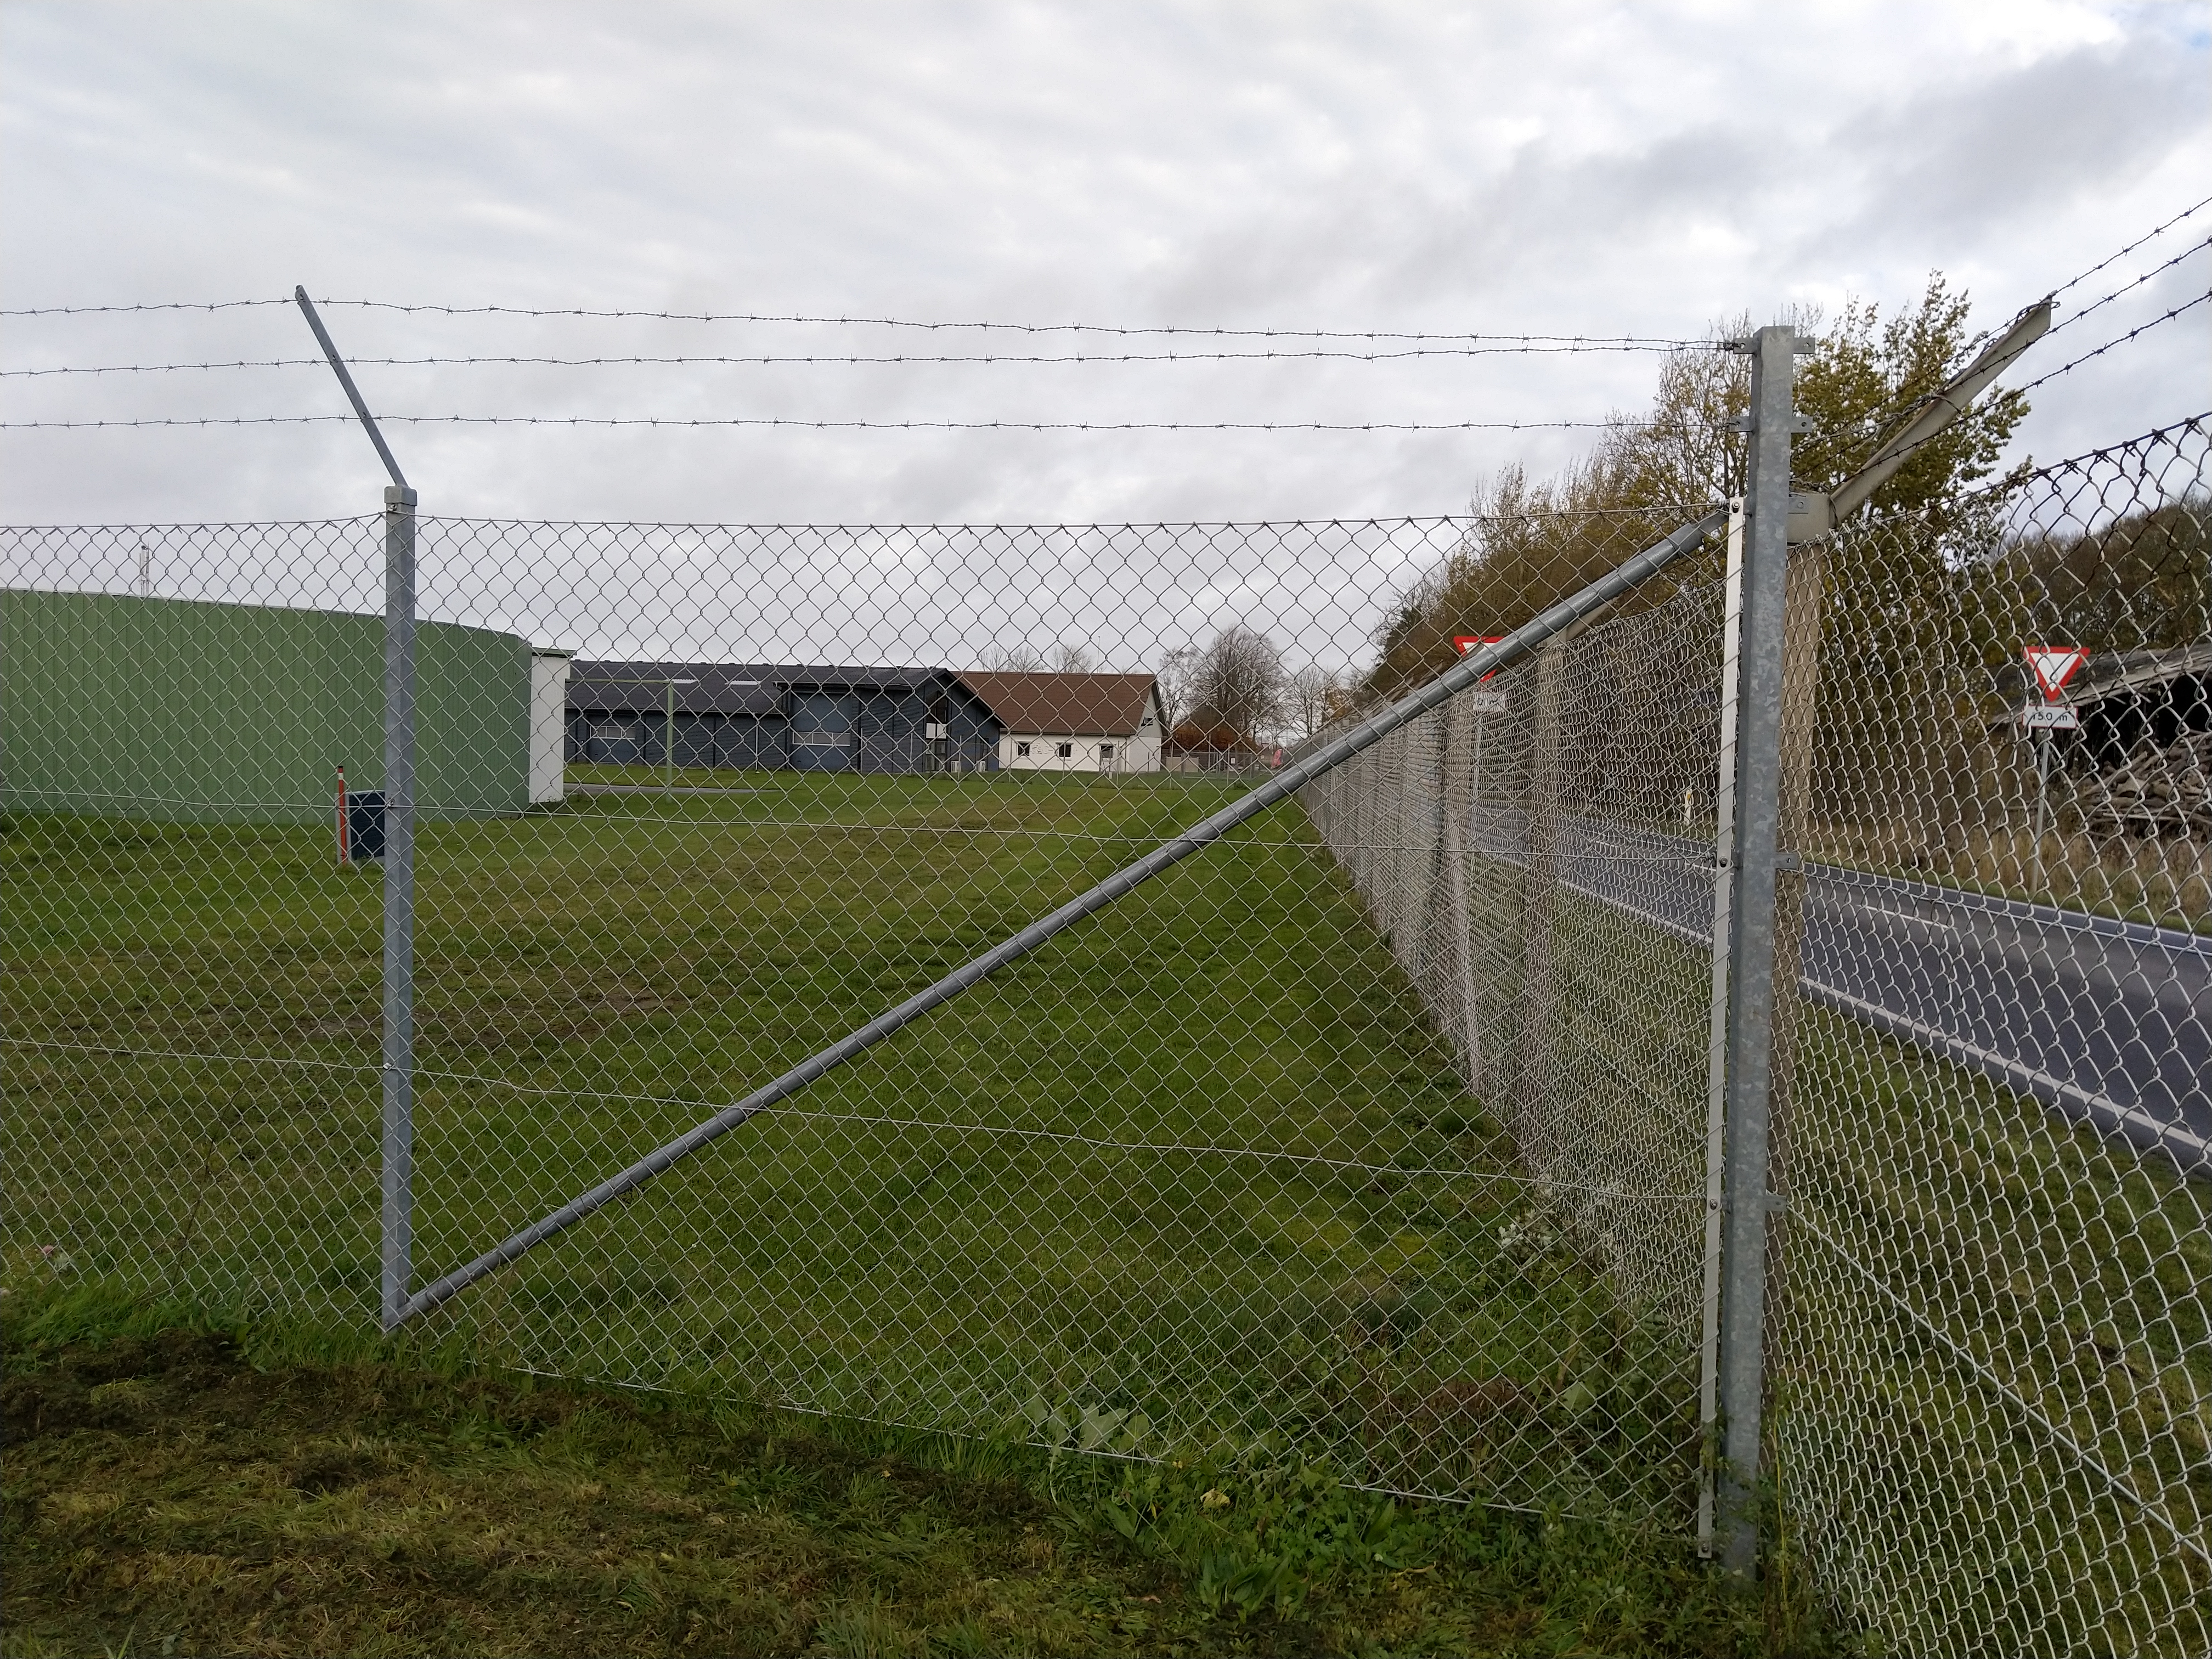
\includegraphics[width=\textwidth]{../Figures/unet_input.pdf}
    \end{subfigure}
    \hfill
    \begin{subfigure}{0.49\textwidth}
        \centering
        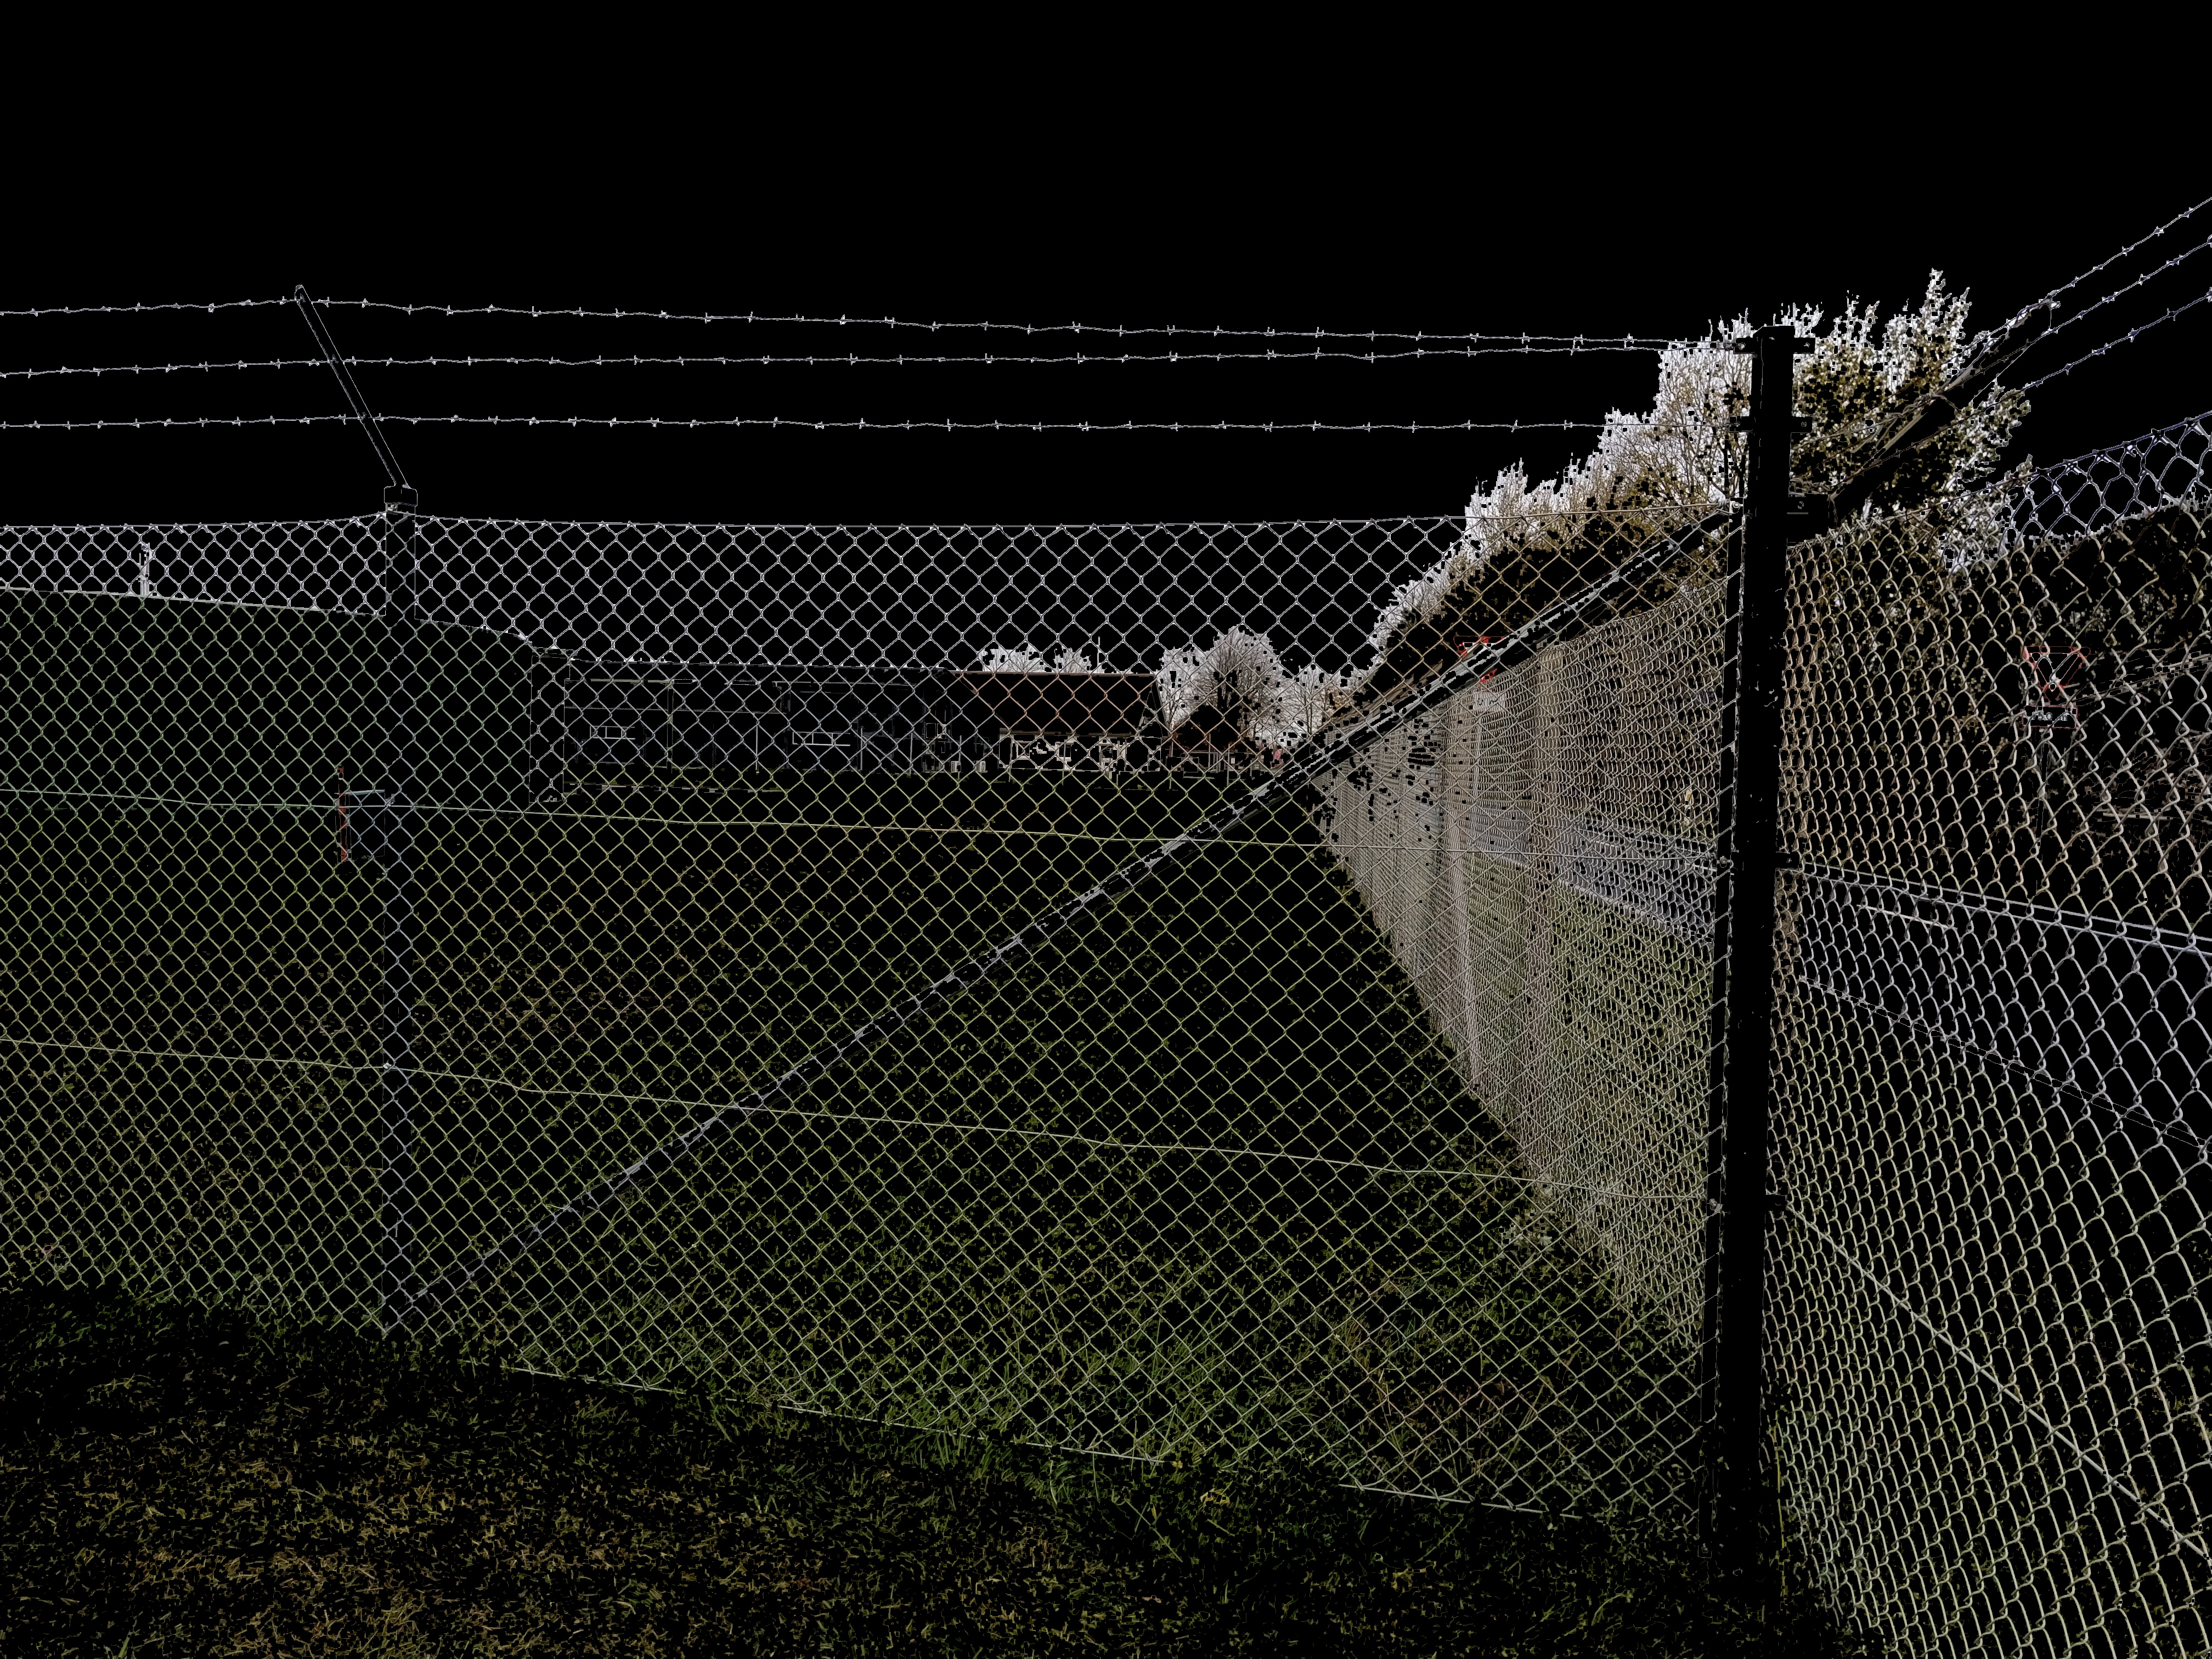
\includegraphics[width=\textwidth]{../Figures/unet_gt.jpg}
    \end{subfigure}
    \caption{U-Net Input Image and Mask}
    \label{fig:unet_input}
\end{figure}

\clearpage
\subsubsection{Convolution based segmentation}
\label{seg:conv_segmentation}
\begin{wrapfigure}{r}{0.35\textwidth}
    \centering
    \vspace{-10pt}
    \includegraphics[width=0.33\textwidth]{../Figures/conv/kernel.png}
    \caption{The kernel used for the method}
    \label{fig:conv_kernel}
\end{wrapfigure}
This method was based on a different idea. Instead of trying to segment the fence structure itself, the intersections in the fence structure would be detected instead resulting in a list of pixel coordinates. A breach detection algorithm could then be developed to find breaches in the structure of pixel locations.\par 
Different approaches was considered but a convolution based solution was chosen. The algorithm would run sequential on each each step based on the blue colour channel. A 33 x 33 kernel was made to generate a high response when being in the center of an intersection. This kernel can be seen as an image in \autoref{fig:conv_kernel}. Black correspond to negative contribution, gray zero and white to positive contribution. This kernel was convoluted with the image to produce a response map featuring high responses were an intersection was found. This image was then normalised to values between 0 and 255 and then thresholded. Contours will then be found in the thresholded image and the centroids of those returned as the final pixel position.\par 

In \autoref{fig:conv_tst0} the different stages of the process can be seen. On the left is the blue colour channel as input, next to that the response from the convolution, then the thresholded image and finally the centroids for the found contours drawn onto the original image.\\
The tuning in this algorithm lies in the thresholding values for the binary thresholding. The methods was tuned to perform its best on the input image.

\begin{figure}[H]
    \centering
    \begin{subfigure}{0.24\textwidth}
        \centering
        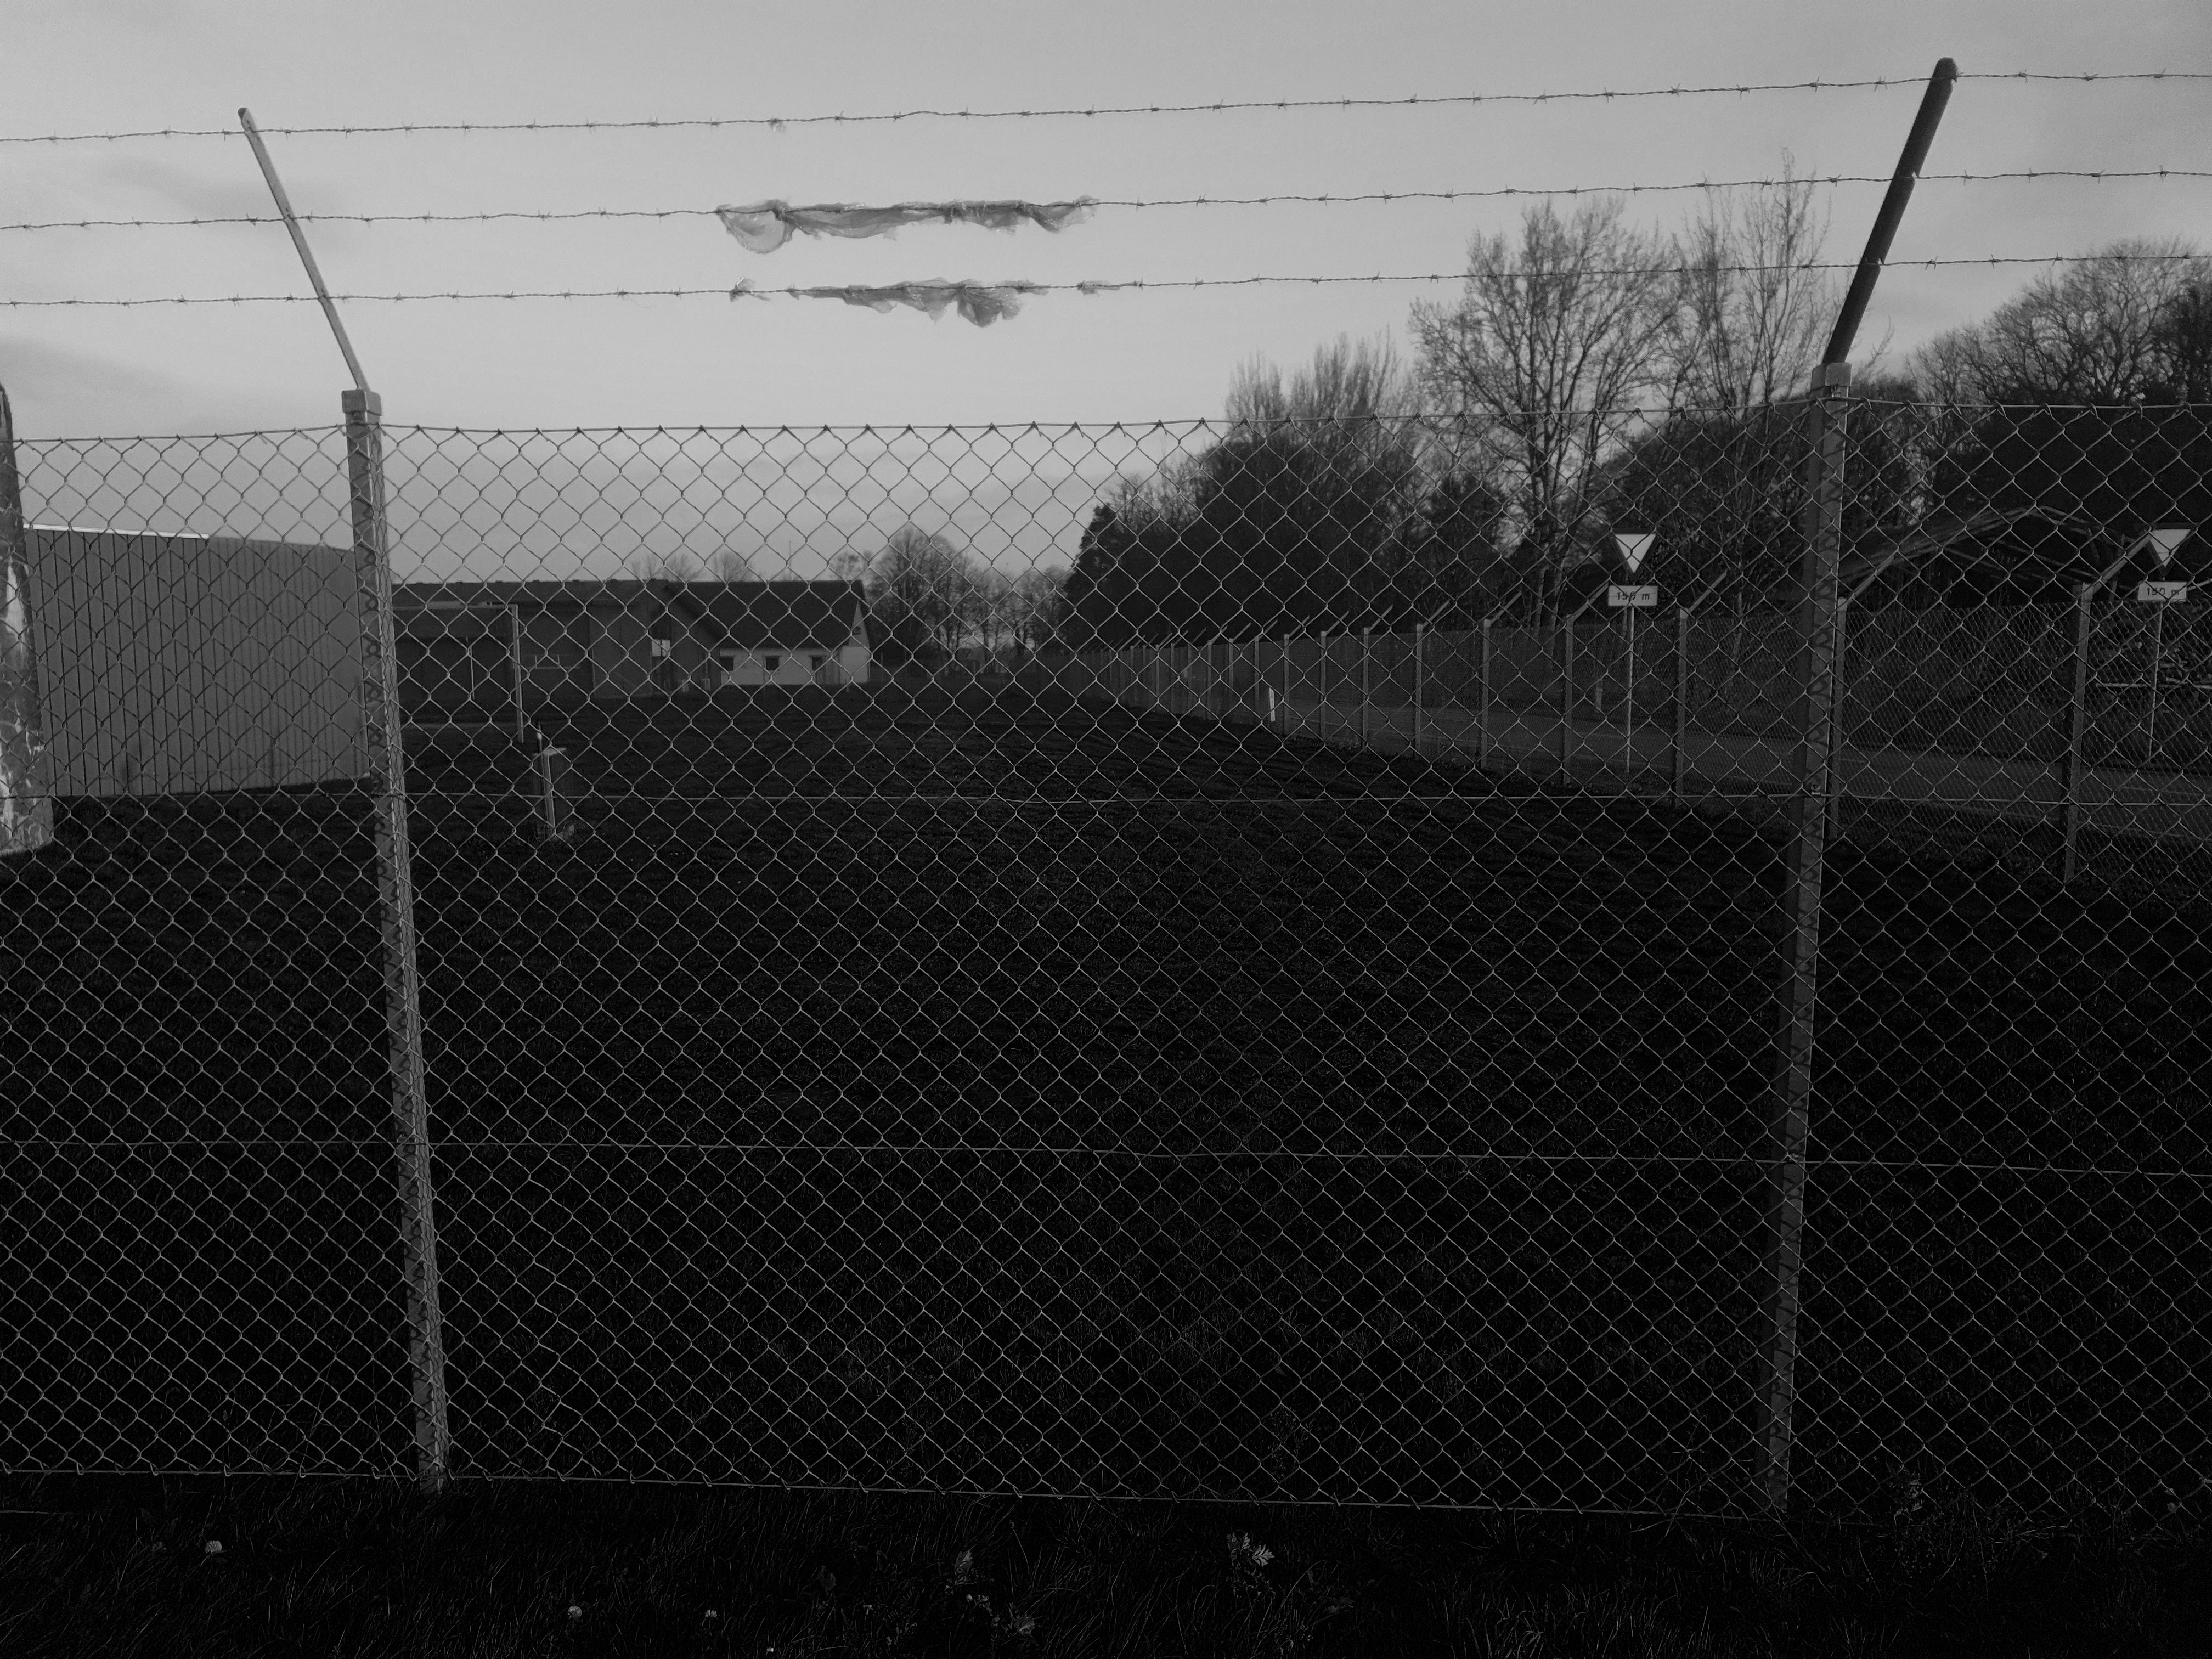
\includegraphics[width=\textwidth]{../Figures/conv/conv_zero/img_zero_blue_channel.jpg}
        \caption{Input blue channel}
        \label{fig:conv_tst0_blue}
    \end{subfigure}
    \hfill
    \begin{subfigure}{0.24\textwidth}
        \centering
        \includegraphics[width=\textwidth]{../Figures/conv/conv_zero/img_one_conv.jpg}
        \caption{Output convolution}
        \label{fig:conv_tst0_conv}
    \end{subfigure}
    \hfill
    \begin{subfigure}{0.24\textwidth}
        \centering
        \includegraphics[width=\textwidth]{../Figures/conv/conv_zero/img_two_threshold.jpg}
        \caption{Output thresholding}
        \label{fig:conv_tst0_thresh}
    \end{subfigure}
    \hfill
    \begin{subfigure}{0.24\textwidth}
        \centering
        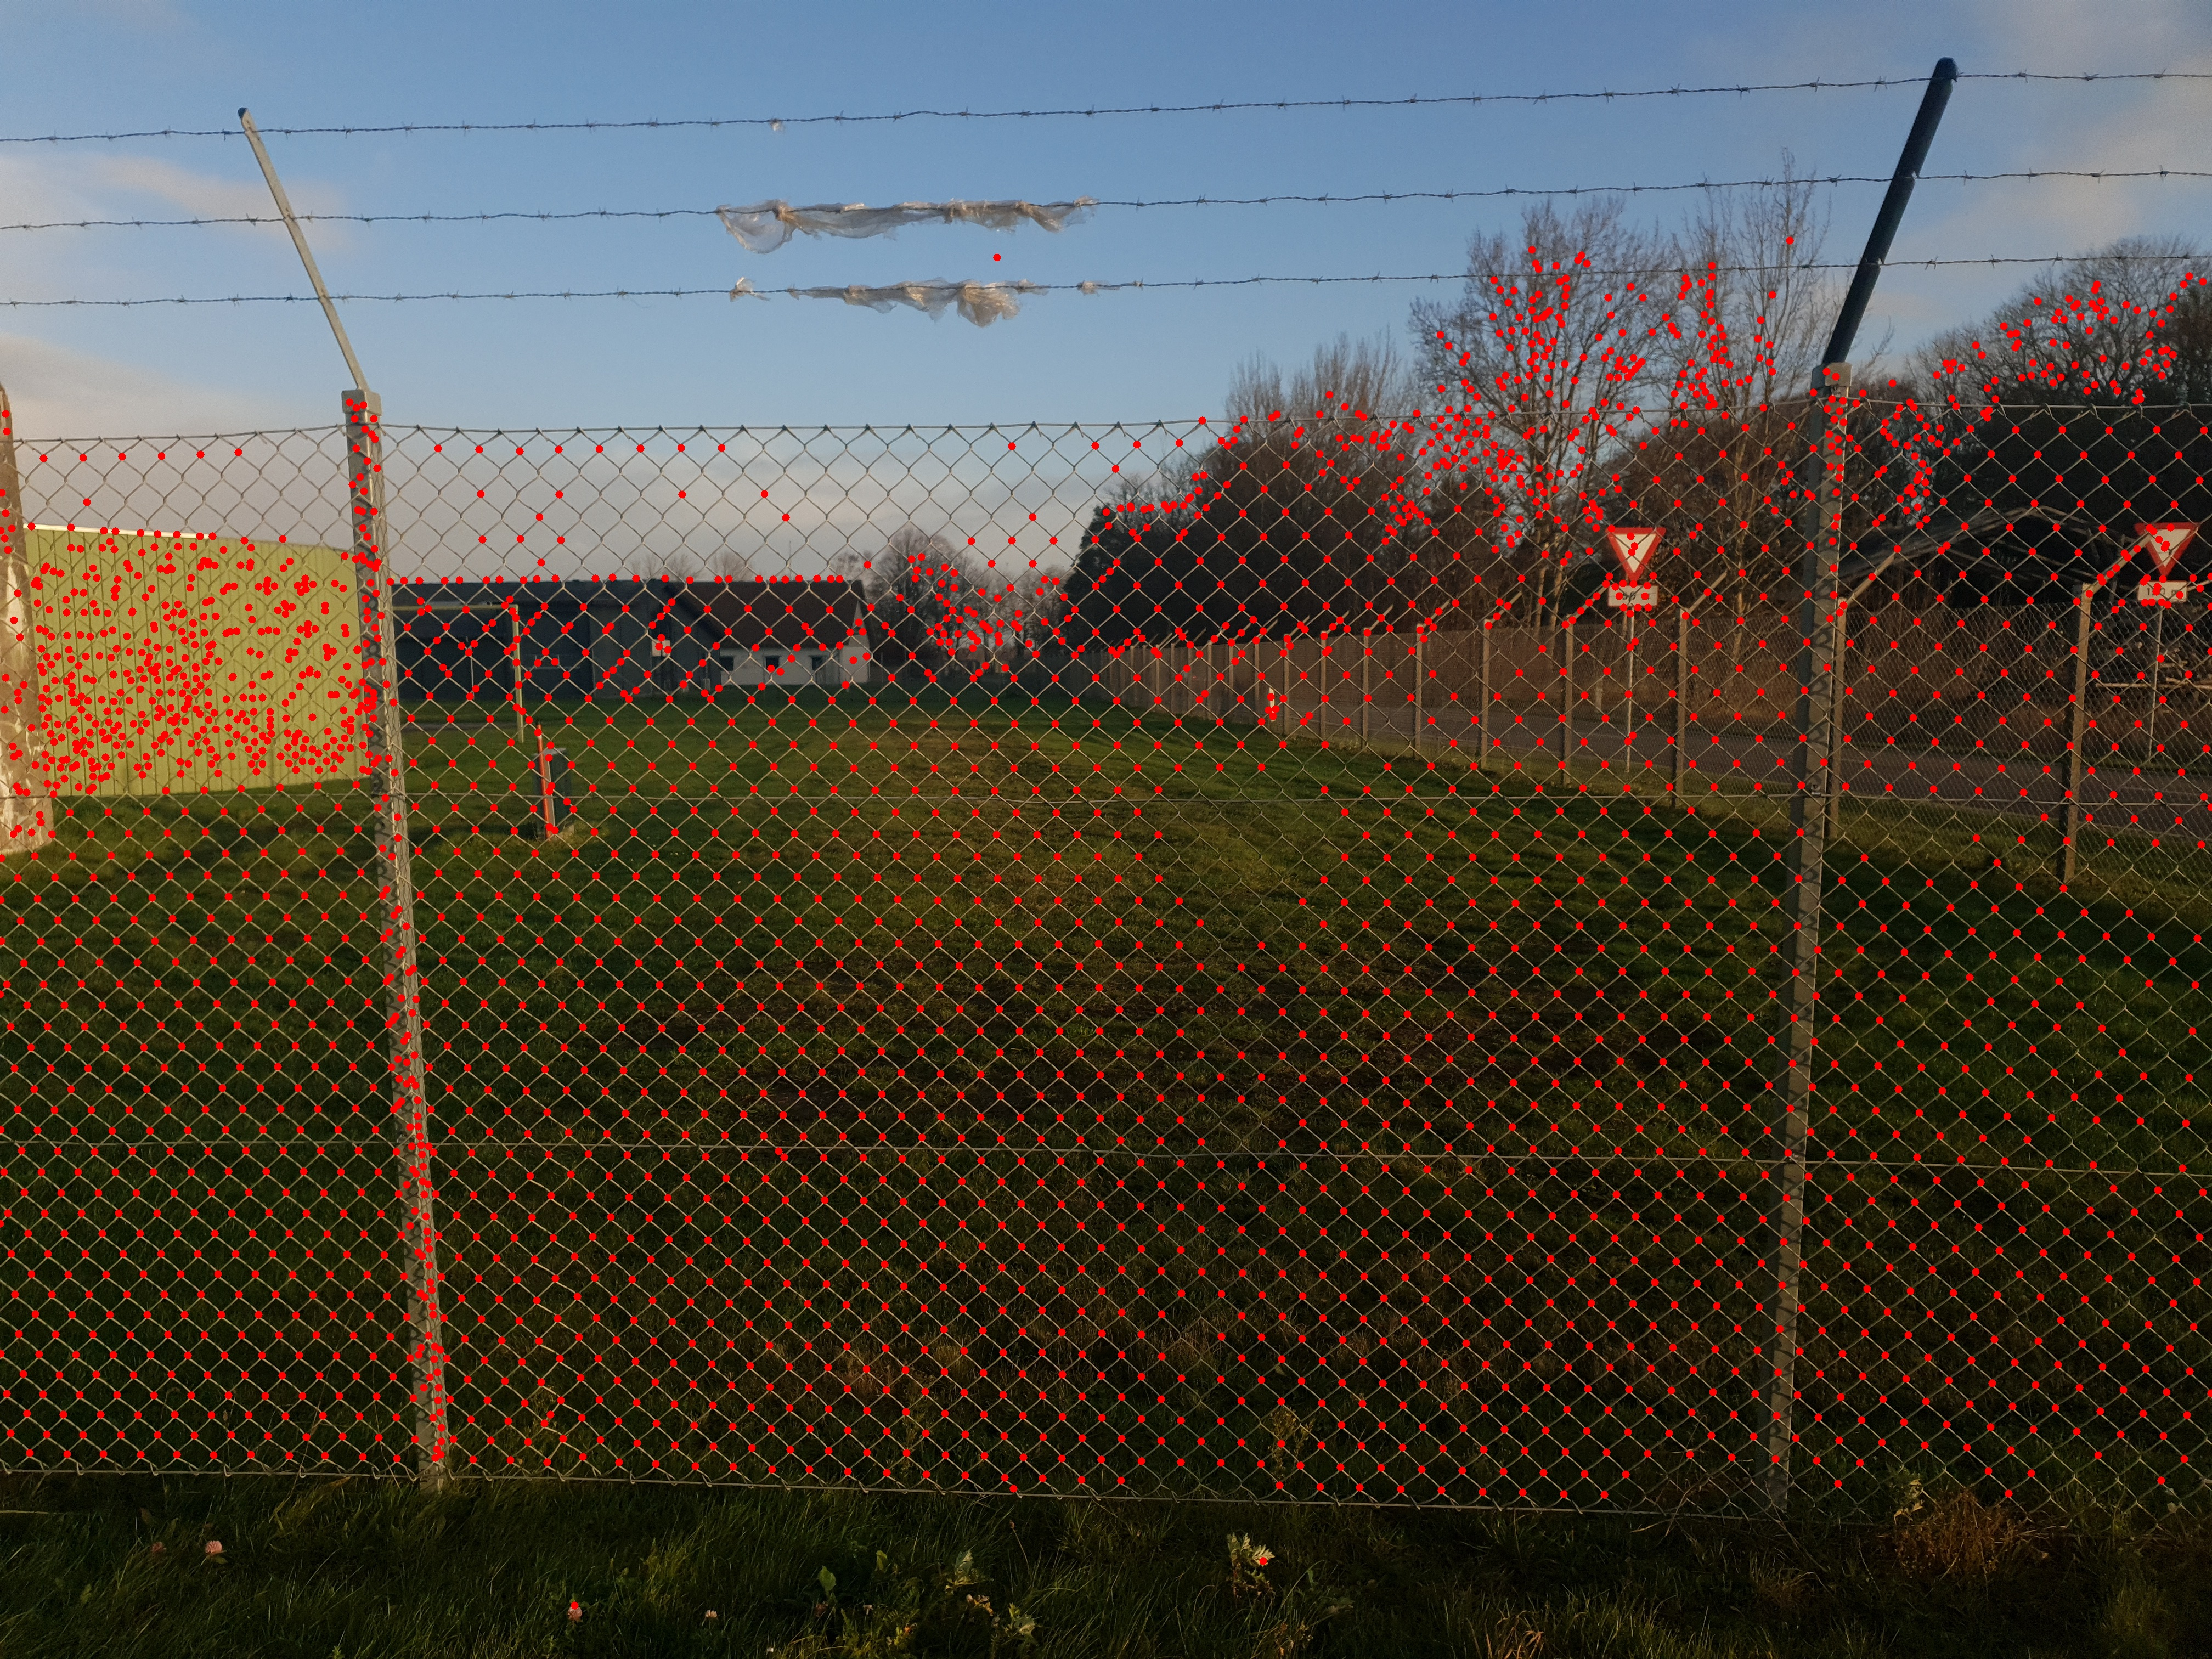
\includegraphics[width=\textwidth]{../Figures/conv/conv_zero/img_three_intersections.jpg}
        \caption{Output pixel positions}
        \label{fig:conv_tst0_px_pos}
    \end{subfigure}
    \caption{Illustration of the processing steps from start to finish}
    \label{fig:conv_tst0}
\end{figure}
\vspace{-15pt}
In \autoref{fig:conv_tst1} another lighter image was run though the method and was again tuned to give the best result. It was generally found that the method were relatively forgiving regarding the thresholds as long as the images were underexposed.

\begin{figure}[H]
    \centering
    \begin{subfigure}{0.24\textwidth}
        \centering
        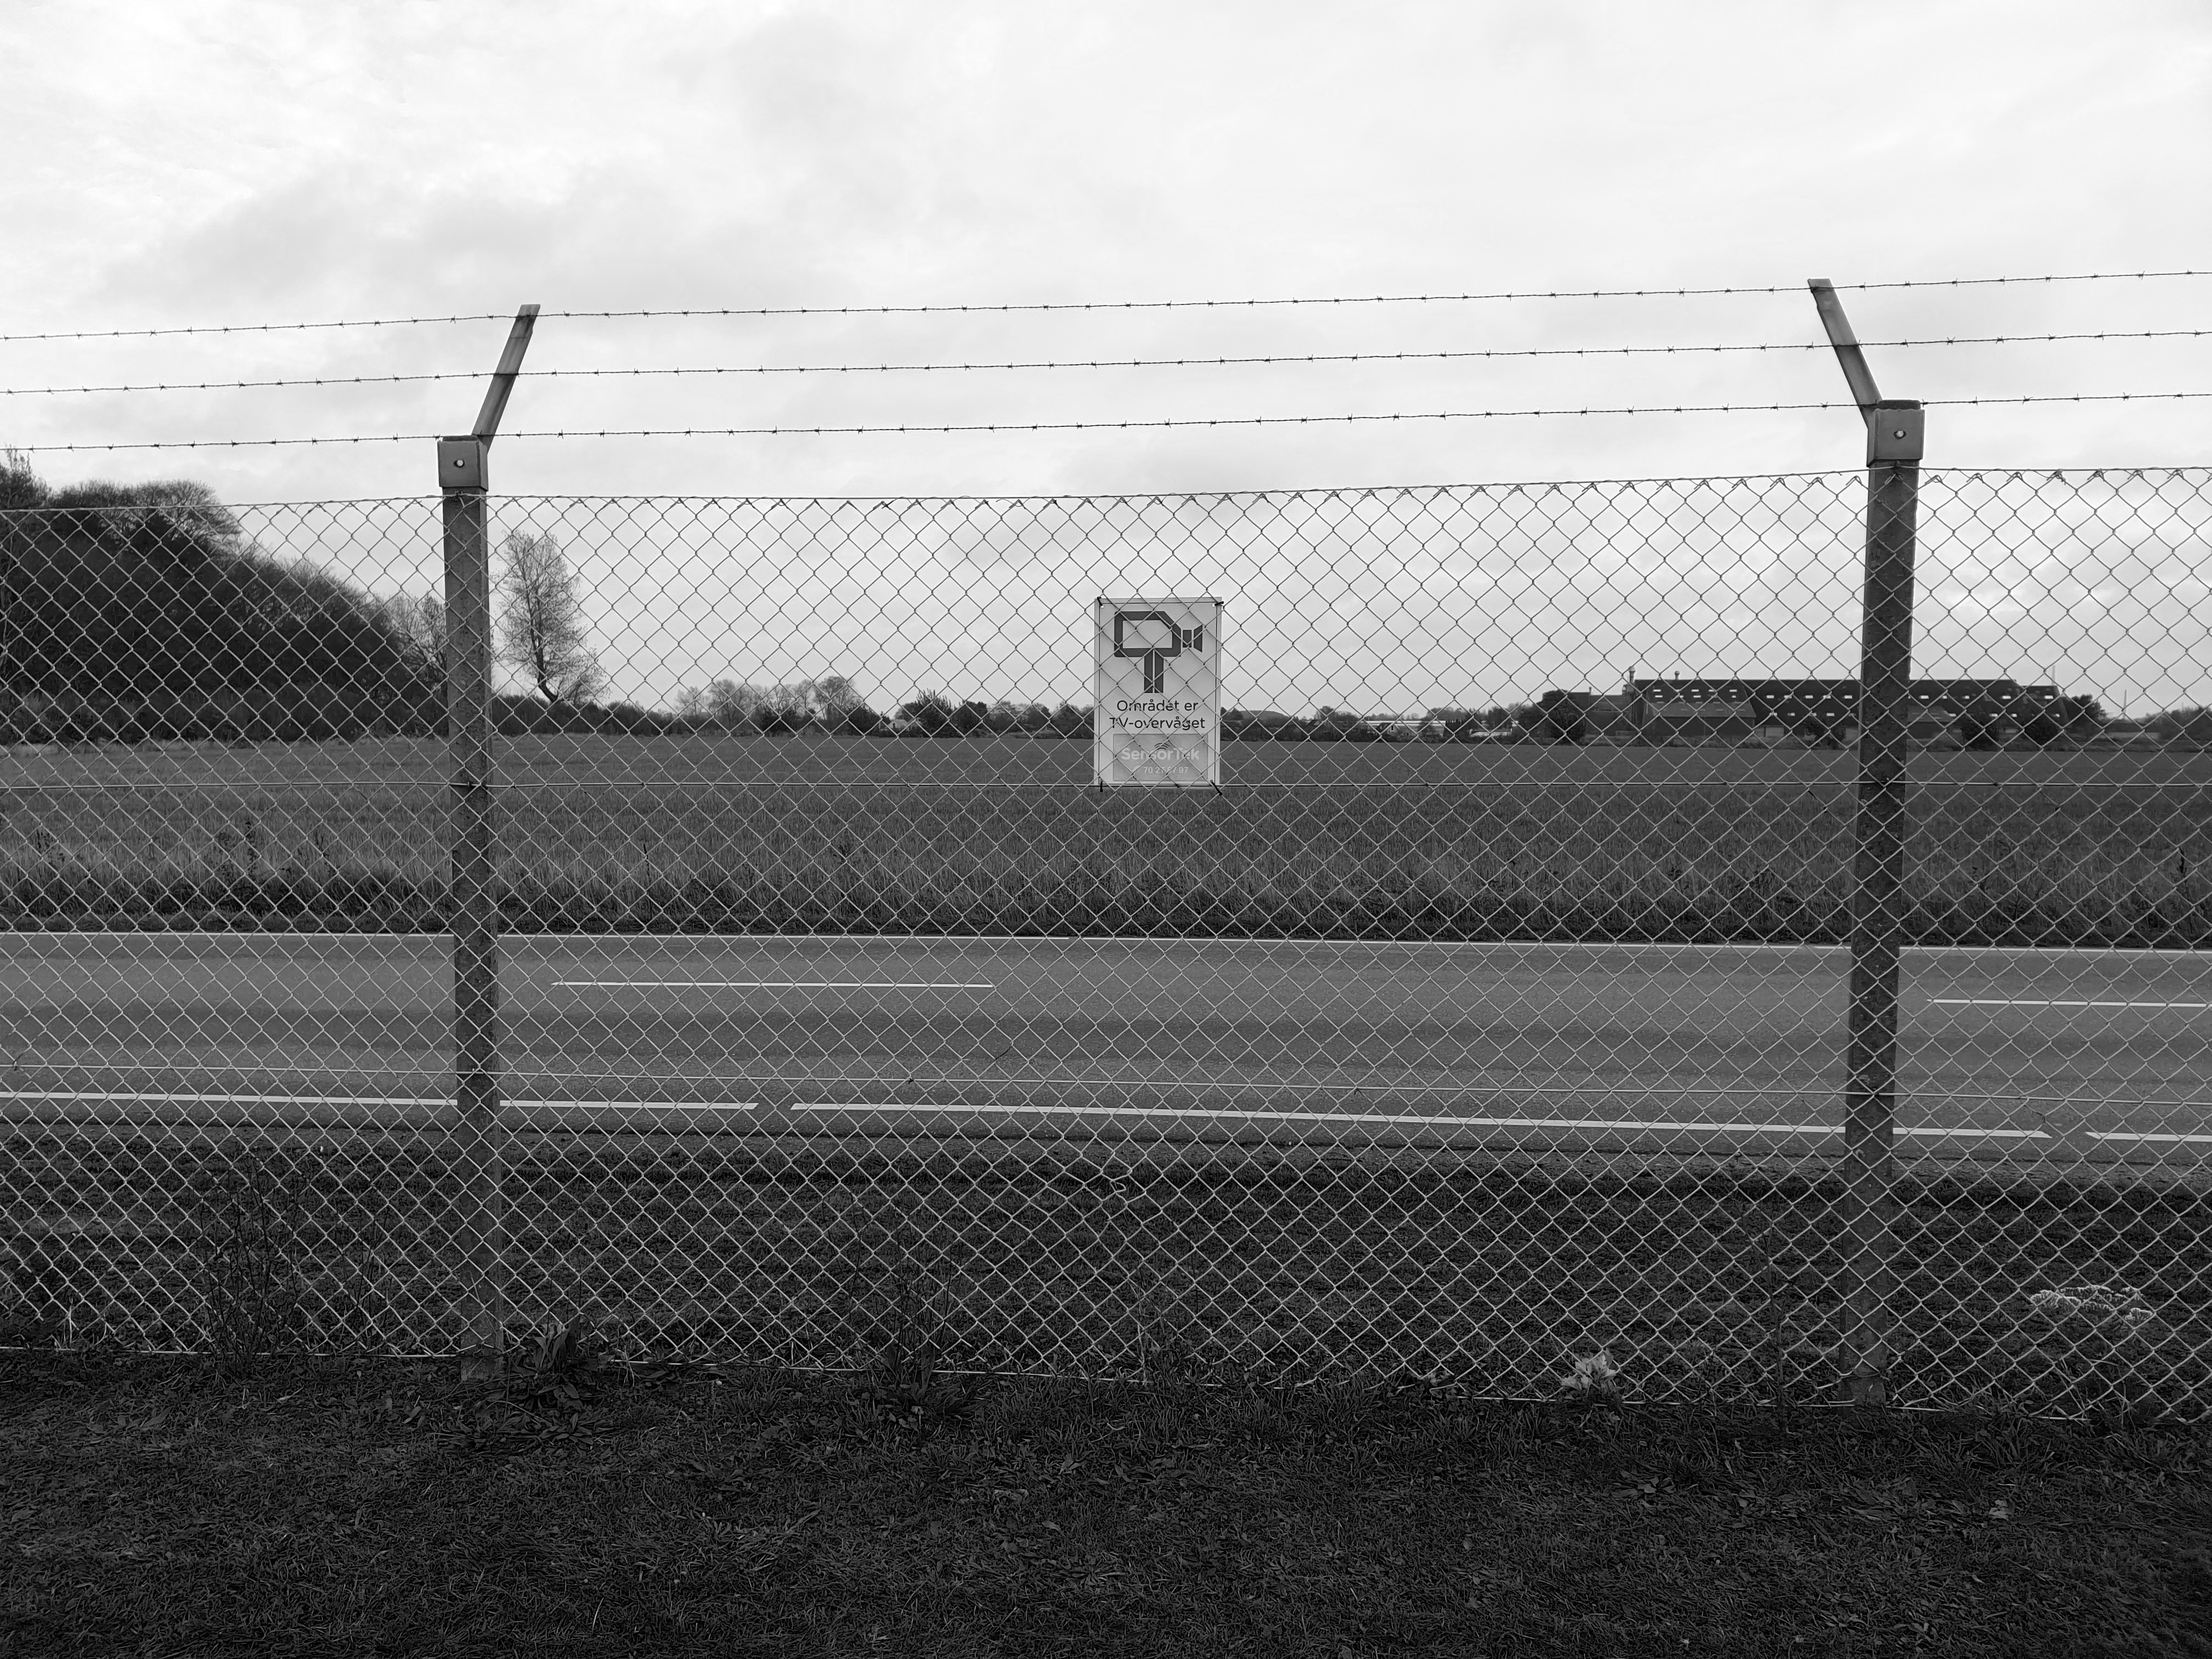
\includegraphics[width=\textwidth]{../Figures/conv/conv_one/img_zero_blue_channel.jpg}
        \caption{Input blue channel}
        \label{fig:conv_tst1_blue}
    \end{subfigure}
    \hfill
    \begin{subfigure}{0.24\textwidth}
        \centering
        \includegraphics[width=\textwidth]{../Figures/conv/conv_one/img_one_conv.jpg}
        \caption{Output convolution}
        \label{fig:conv_tst1_conv}
    \end{subfigure}
    \hfill
    \begin{subfigure}{0.24\textwidth}
        \centering
        \includegraphics[width=\textwidth]{../Figures/conv/conv_one/img_two_threshold.jpg}
        \caption{Output thresholding}
        \label{fig:conv_tst1_thresh}
    \end{subfigure}
    \hfill
    \begin{subfigure}{0.24\textwidth}
        \centering
        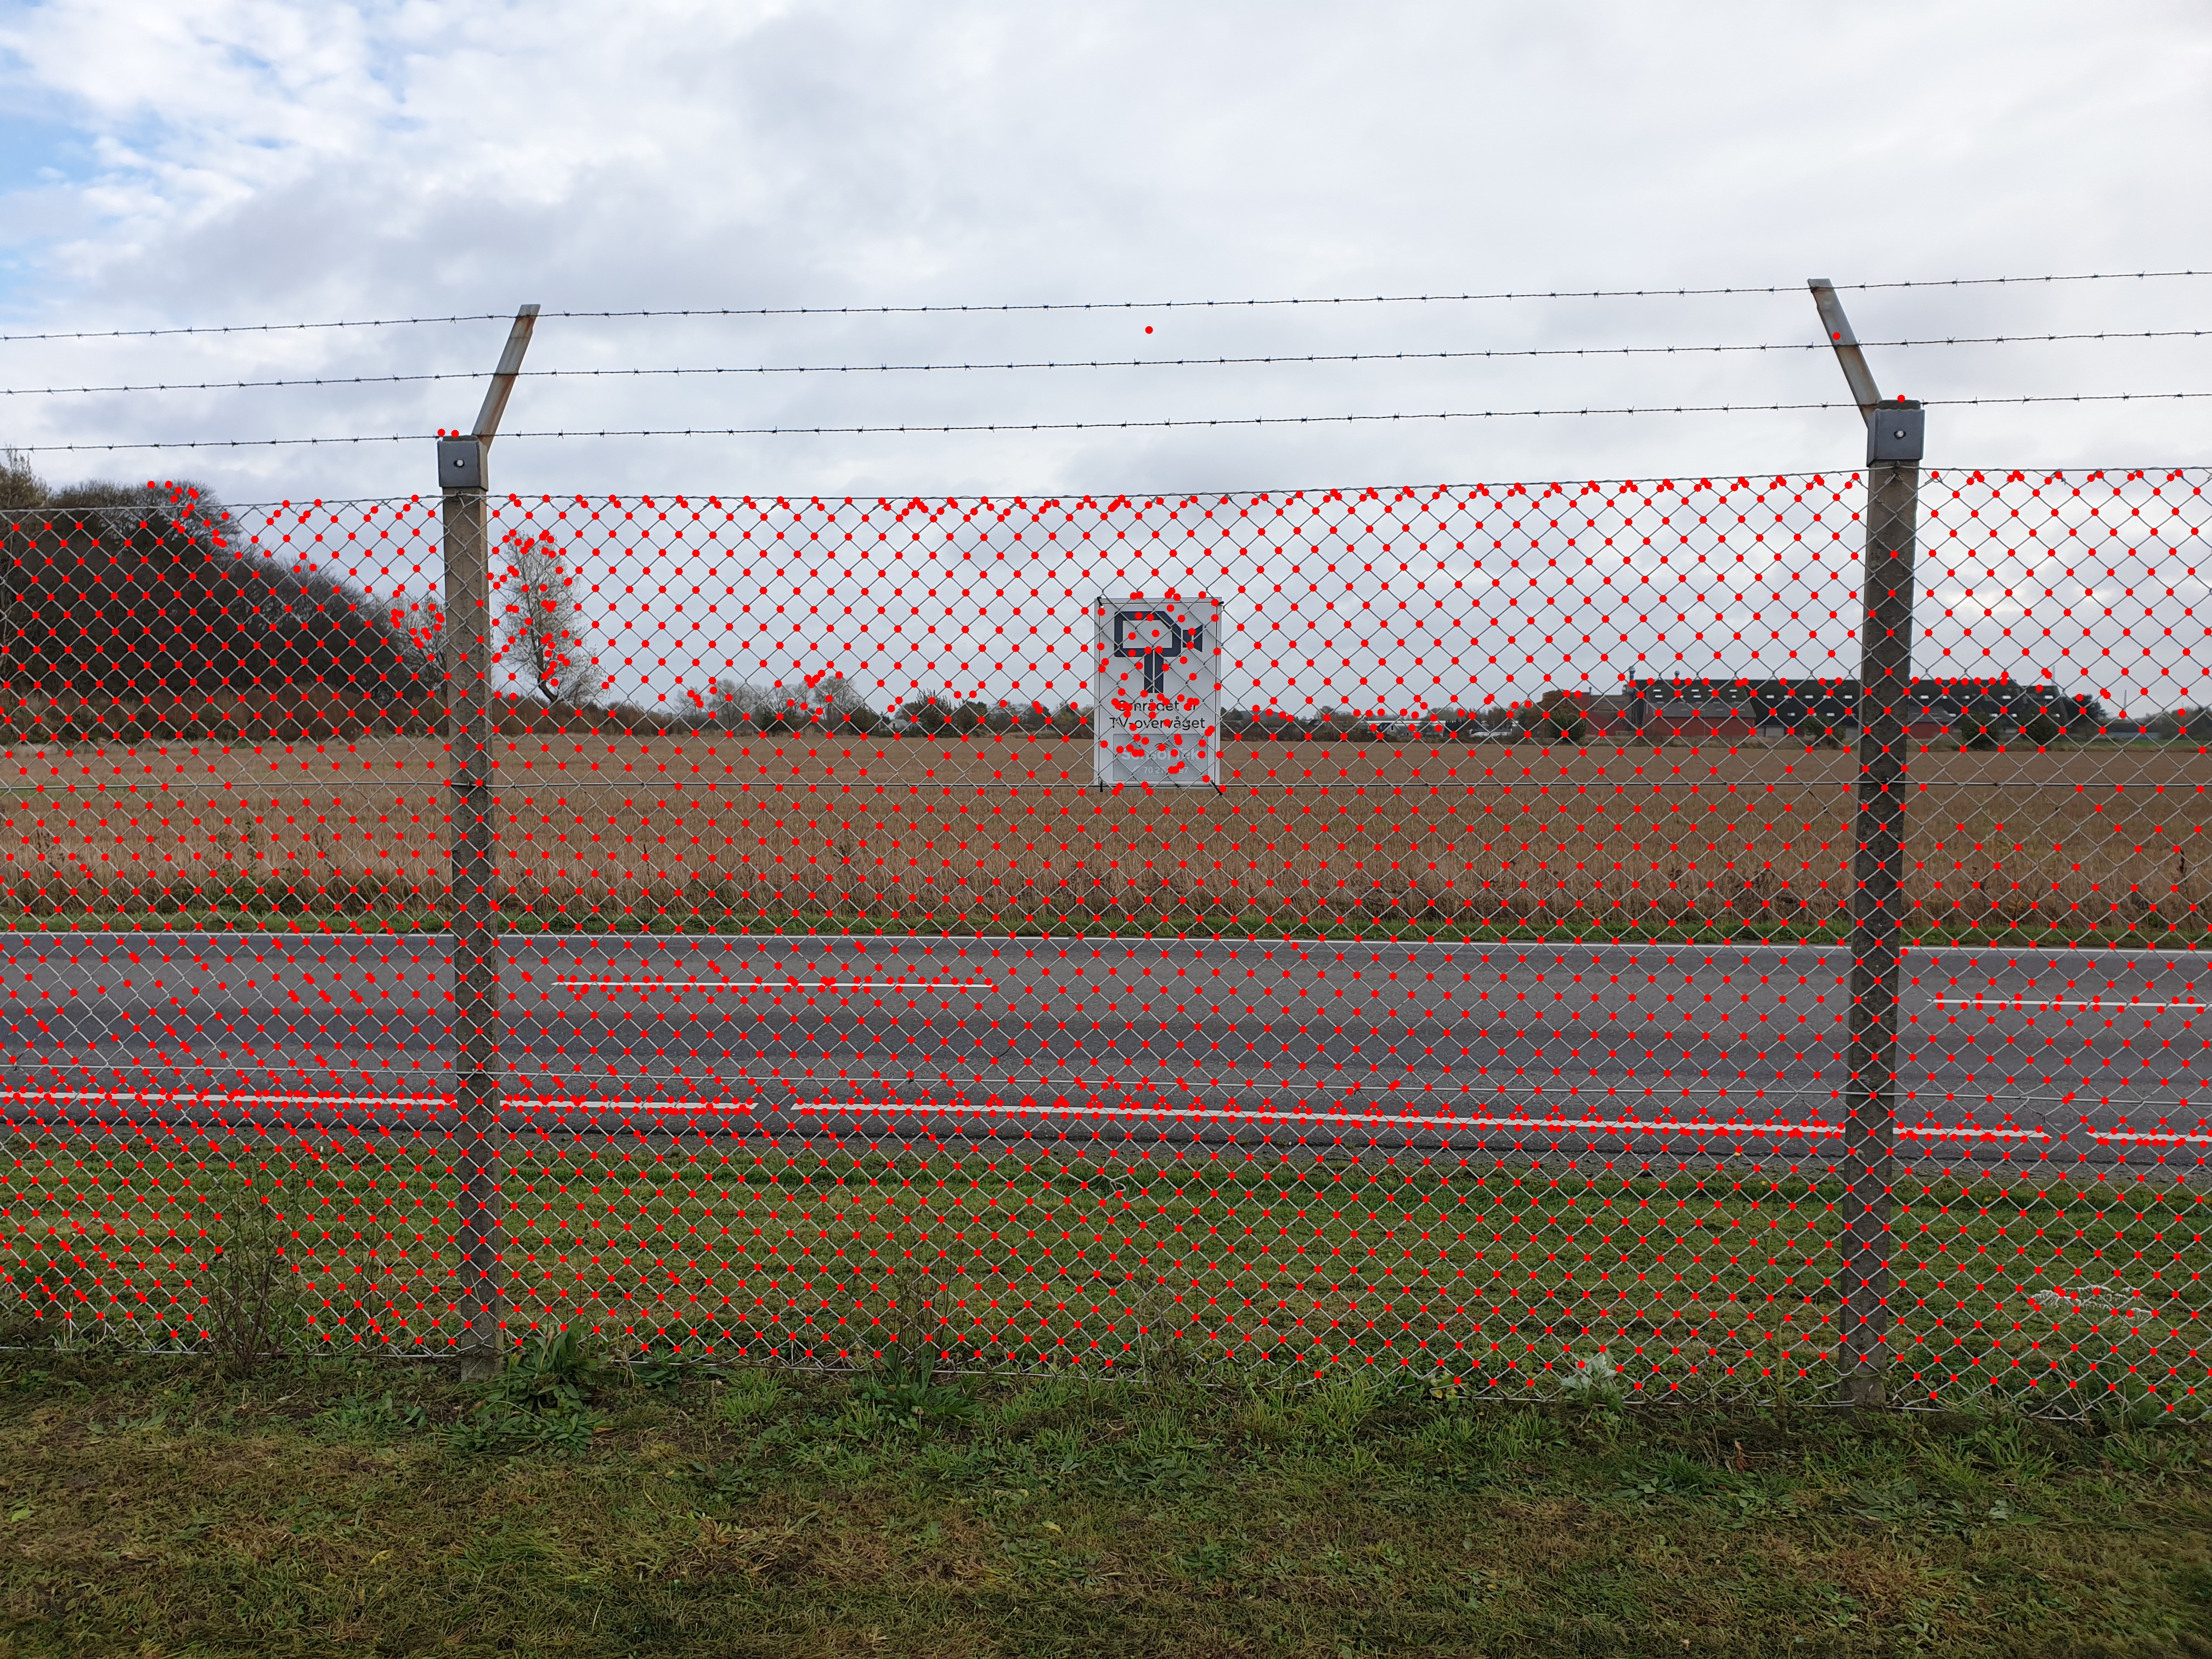
\includegraphics[width=\textwidth]{../Figures/conv/conv_one/img_three_intersections.jpg}
        \caption{Output pixel positions}
        \label{fig:conv_tst1_px_pos}
    \end{subfigure}
    \caption{Illustration of the processing steps from start to finish}
    \label{fig:conv_tst1}
\end{figure}
\vspace{-15pt}
The method handled grass really well but struggled a bit with tress. The result from this would need some filtering of the found points to be useful for detecting breaches.\par
It was considered to maybe connect the points with lines to produce a perfect grid structure that could then be passed to the breach detection algorithm described in \autoref{subsec:screening_for_breaches}.

\subsection{Breach detection}

\subsubsection{Screening of segmented images}
\label{subsec:screening_for_breaches}

Given segmented images where the background has been removed with only the foreground (fence) left in the image, the resulting image can be screened for possible breaches. This is done using an algorithm with the following three stages namely \textit{searching for a fence}, \textit{fence following} and \textit{peak and endpoint detection}. The peaks (junctions) is defined as the intersections where the elements of the fence meets to form a junction. This is the midpoint of the images seen in Figure \ref{fig:fence_search}. 

The basic idea is to find the fence starting from a random location in the middle of the image. The pointer can move in an either up-right, down-right, down-left or up-left direction. This is done so that the pointer initially ends up on the structure on the fence, which it now can follow. This is illustrated in Figure \ref{fig:fence_search} where the fence is white, background black and the pointer labelled blue.    

\begin{figure}[H]
    \centering
    \begin{subfigure}{.24\textwidth}
        \centering
        \includegraphics[width=\textwidth]{../Figures/screening_algorithm/fence_search_step1.png}
        \caption{Step one}
        \label{fig:fence_search_step1}
    \end{subfigure}
    \hfill
    \begin{subfigure}{.24\textwidth}
        \centering
        \includegraphics[width=\textwidth]{../Figures/screening_algorithm/fence_search_step2.png}
        \caption{Step two}
        \label{fig:fence_search_step2}
    \end{subfigure}
    \hfill
    \begin{subfigure}{.24\textwidth}
        \centering
        \includegraphics[width=\textwidth]{../Figures/screening_algorithm/fence_search_step3.png}
        \caption{Step three}
        \label{fig:fence_search_step3}
    \end{subfigure}
    \hfill
    \begin{subfigure}{.24\textwidth}
        \centering
        \includegraphics[width=\textwidth]{../Figures/screening_algorithm/fence_search_step4.png}
        \caption{Step four}
        \label{fig:fence_search_step4}
    \end{subfigure}
    \caption{Illustration of searching for a fence in the image. Fence (white), background (black), white arrows (illegal stopping criteria) and black arrows (valid stopping criteria)}
    \label{fig:fence_search}
\end{figure}

The pointer continues to move in a certain direction until the giving pixel value is above a threshold. When this happens, the pointer will now move in either two directions which is orthogonal to the last move direction. This can be seen in Figure \ref{fig:line_search}. Now the pointer moves in a direction with a chosen step size for each move. The step size can be given as a list of values so that the pointer can move further away from its last position in each step. This is done to take into account low pixel values in the next step even thought the pointer is still on the fence. Moreover, the next step of the pointer can be moved in orthogonal directions according to the last move if an abnormal fence structure is seen like the one in Figure \ref{fig:abnormal_fence_strcuture}. 

\begin{figure}[H]
    \centering
    \begin{subfigure}{.22\textwidth}
        \centering
        \includegraphics[width=\textwidth]{../Figures/screening_algorithm/line_search_step1.png}
        \caption{Step one}
        \label{fig:line_search_step1}
    \end{subfigure}
    \hfill
    \begin{subfigure}{.22\textwidth}
        \centering
        \includegraphics[width=\textwidth]{../Figures/screening_algorithm/line_search_step2.png}
        \caption{Step two}
        \label{fig:line_search_step2}
    \end{subfigure}
    \hfill
    \begin{subfigure}{.22\textwidth}
        \centering
        \includegraphics[width=\textwidth]{../Figures/screening_algorithm/line_search_step3.png}
        \caption{Step three}
        \label{fig:line_search_step3}
    \end{subfigure}
    \hfill
    \begin{subfigure}{.245\textwidth}
        \centering
        \includegraphics[width=\textwidth]{../Figures/screening_algorithm/abnormal_fance_structure.png}
        \caption{Abnormal fence structure}
        \label{fig:abnormal_fence_strcuture}
    \end{subfigure}
    \caption{Illustration of the line (fence) follower approach. Fence (white), background (black), white arrows (illegal stopping criteria) and black arrows (valid stopping criteria)}
    \label{fig:line_search}
\end{figure}

\clearpage
The pointer will continue to move until a peak location or end of fence is seen based on the pixel values. The way the algorithm detects peaks is illustrated in Figure \ref{fig:peak_search}. At every step in the fence following approach the algorithm will check for high pixel values in front of it as well as its orthogonal directions according to the last move. If the pixel value in all three directions is above a threshold it will be considered to be a peak location. The point in the image coordinates will be put on a list of already detected peak points. Now the algorithm will branch in the other directions at the peak location to continue its search for peaks and endpoints. This can be done either in an recursive or iterative manor.    

\begin{figure}[H]
    \centering
    \begin{subfigure}{.24\textwidth}
        \centering
        \includegraphics[width=\textwidth]{../Figures/screening_algorithm/peak_search_step1.png}
        \caption{Step one}
        \label{fig:peak_search_step1}
    \end{subfigure}
    \hfill
    \begin{subfigure}{.24\textwidth}
        \centering
        \includegraphics[width=\textwidth]{../Figures/screening_algorithm/peak_search_step2.png}
        \caption{Step two}
        \label{fig:peak_search_step2}
    \end{subfigure}
    \hfill
    \begin{subfigure}{.24\textwidth}
        \centering
        \includegraphics[width=\textwidth]{../Figures/screening_algorithm/peak_search_step3.png}
        \caption{Step three}
        \label{fig:peak_search_step3}
    \end{subfigure}
    \hfill
    \begin{subfigure}{.24\textwidth}
        \centering
        \includegraphics[width=\textwidth]{../Figures/screening_algorithm/peak_search_step4.png}
        \caption{Step four}
        \label{fig:peak_search_step4}
    \end{subfigure}
    \caption{Illustration of searching for a peak (junction) in the fence.  Fence (white), background (black), white arrows (illegal stopping criteria) and black arrows (valid stopping criteria)}
    \label{fig:peak_search}
\end{figure}
\vspace{-15pt}
Endpoints is detected if the fence following part of the algorithm sees only black pixels (pixels below a threshold) in the next steps to come. Hence, the algorithm will return from its given branch and put the endpoint on a list to be used in the analysis of breaches in a later step.\\
To make the algorithm faster a region of interest (ROI) was defined which can be seen in Figure \ref{fig:screening_algorihtm}. The recursion will stop if it goes beyond the ROI. As it can be seen, large custom made breaches can be found and small breaches or noise are neglected. The endpoints inside the ROI is grouped together using hierarchical clustering. This approach finds the distance between points. It will group points based on the distance from a given point to that of the mean of a cluster. This is both a fast and effective method in order to cluster points and make an approximation of the size of the breach knowing the cluster diameter.     

\begin{figure}[H]
    \centering
    \begin{subfigure}{.49\textwidth}
        \centering
        \includegraphics[width=\textwidth]{../Figures/screening_algorithm/fence_clean_peaks.png}
        \caption{Fence without breaches}
        \label{fig:screening_clean_peaks}
    \end{subfigure}
    \begin{subfigure}{.49\textwidth}
        \centering
        \includegraphics[width=\textwidth]{../Figures/screening_algorithm/fence_breach_peaks.png}
        \caption{Fence with custom made breaches}
        \label{fig:screening_breaches_peaks}
    \end{subfigure}
    \caption{Illustration of screening a fence given images from the Fourier transformation. Peaks (blue), breaches (red), neglected small breaches or noise (green) and ROI (white)}
     \label{fig:screening_algorihtm}
\end{figure}
\vspace{-15pt}
The algorithm performs quite well given a nicely segmented input image. However, because the implementation is based of the need of a really good segmented input image, the algorithm will fail if the input is bad e.g. given a bad segmented image from the Fourier transformation. This is due to the fact that the pointer will follow the structure of the fence, but if the fence is badly segmented from the background, this algorithm will not work. 

In theory, it is possible to find very small breaches using this screening approach of the image because it tries to find every peak and endpoint location in the image. The limitations is based on the need for a perfectly segmented input image.  

\subsubsection{Image classification and boundary box regression using mask-RCNN}
\label{subsec:deep_learning_cnn}

A number of algorithms where taken into consideration in regard to deep learning. Faster-RCNN is an extension of the region-based convolution neural network (RCNN). The RCNN uses the selective search algorithm to extract proposal regions from the image from where these are given to a convolution neural network (CNN) which extracts a feature vector from the regions in question. Then these are given to a set of class specific support vector machines (SVM) where classification and offsets to boundary box regression is performed. Instead of using the selective search algorithm, the faster-RCNN makes a convolution feature map from the input image using a convolution network. A separate network is then used to find region proposals. This predicted region is reshaped using a region of interest pooling layer to classify the picture being within the proposed region and offsets values for the giving boundary boxes. \textbf{Mask-RCNN}, Figure \ref{fig:faster_rcnn}, extends to this idea by adding an additional branch being the objects mask. This enables the possibility to make instance segmentation to the found objects.\cite{FasterRCNN} \cite{MaskRCNN} \cite{prosConsDeepLearning}

\begin{figure}[H]
    \centering
    \begin{subfigure}[t]{.30\textwidth}
        \centering
        \includegraphics[width=\textwidth]{../Figures/deep_learning_algorithms/faster_rcnn.png}
        \caption{The faster-RCNN algorithm \cite{FasterRCNN}}
        \label{fig:faster_rcnn}
    \end{subfigure}
        \begin{subfigure}[t]{.43\textwidth}
        \centering
        \includegraphics[width=\textwidth]{../Figures/deep_learning_algorithms/yolo.png}
        \caption{The YOLO algorithm\cite{prosConsDeepLearning}}
        \label{fig:yolo}
    \end{subfigure}
    \caption{Illustrations of the considered algorithms to use in deep learning}
     \label{fig:considered_algorihtms_deep_learning}
\end{figure}

In \textbf{YOLO} (you only look ones), Figure \ref{fig:yolo}, an image is split up into grids of size $N \times N$ where each grid consists of $m$ bounding boxes. It uses a CNN to predict bounding boxes and class probabilities for each box. This algorithm is quite fast, but its comes with the expense of bad detection of small objects.

Given these methods it has been decided to move on with the Mask-RCNN because the precision is preferred instead of speed and the possibility of using the instance segmentation for estimating the size of the breach in the given image.

\subsubsection*{Data augmentation}
In order to train the network a lot of data have to be collected in order to make a robust solution. Shared data from group 171 in the experts in teams course has been used. This data represents a lot of images where a 3D-model of a fence with artificial breaches has been placed in front of different backgrounds as seen in Figure \ref{fig:custom_fence_one}, \ref{fig:custom_fence_two} and \ref{fig:custom_fence_three}. This includes almost 500 images with fences in different configurations. However, more images are needed, so data augmentation is used. The augmented data takes into account different conditions like weather, lightening, blur and noise in the image. This has been done automatically in python where 15 new images have been made from each original image. Every image has been scaled and blurred differently each time. Moreover, rain, snow, fog, Gaussian noise and perspective transformations has randomly been given to each of these images. The result of three of them can be seen in Figure \ref{fig:custom_snow}, \ref{fig:custom_rain} and \ref{fig:custom_fog}.

\begin{figure}[H]
    \centering
    \begin{subfigure}{.3\textwidth}
        \centering
        \includegraphics[width=\textwidth]{../Figures/augmentations/img_bb30.png}
        \caption{Custom fence one}
        \label{fig:custom_fence_one}
    \end{subfigure}
    \hfill
    \begin{subfigure}{.3\textwidth}
        \centering
        \includegraphics[width=\textwidth]{../Figures/augmentations/img_bb60.png}
        \caption{Custom fence two}
        \label{fig:custom_fence_two}
    \end{subfigure}
    \hfill
    \begin{subfigure}{.3\textwidth}
        \centering
        \includegraphics[width=\textwidth]{../Figures/augmentations/img_bb150.png}
        \caption{Custom fence three}
        \label{fig:custom_fence_three}
    \end{subfigure}
    \hfill
    \begin{subfigure}{.3\textwidth}
        \centering
        \includegraphics[width=\textwidth]{../Figures/augmentations/img_bb35.png}
        \caption{Custom snow}
        \label{fig:custom_snow}
    \end{subfigure}
    \hfill
    \begin{subfigure}{.3\textwidth}
        \centering
        \includegraphics[width=\textwidth]{../Figures/augmentations/img_bb62.png}
        \caption{Custom rain}
        \label{fig:custom_rain}
    \end{subfigure}
    \hfill
    \begin{subfigure}{.3\textwidth}
        \centering
        \includegraphics[width=\textwidth]{../Figures/augmentations/img_bb161.png}
        \caption{Custom fog}
        \label{fig:custom_fog}
    \end{subfigure}
    \caption{Illustration of some of the custom made fences with different backgrounds. The original form can be seen in Figure \ref{fig:custom_fence_one}, \ref{fig:custom_fence_two}, \ref{fig:custom_fence_three} and its augmented parts in Figure \ref{fig:custom_snow}, \ref{fig:custom_rain} and \ref{fig:custom_fog} respectively }
     \label{fig:custom_fences_with_augmentation}
\end{figure}
\vspace{-15pt}
The data augmentation resulted in almost 7000 new images which is going to be used for training the deep neural network (DNN). 80\% of the images will be used for training and 20\% as validation/test images. The augmentation with snow, rain and fog has been used to take into account real life scenarios when the drone has to fly in different whether conditions and still make a robust estimation of possible breaches in the fences. \cite{imgaug}  

\subsubsection*{Mask-RCNN}

Mask-RCNN consist of two stages. The first stage begins with the bottom up path where a computation of the backbone (ResNet101 in this implementation) to compute a hierarchy of features at different scales with a scaling factor of two. This is denoted as \textit{C2} (conv2), \textit{C3} (conc3), \textit{C4} (conv4) and \textit{C5} (conv5) in Figure \ref{fig:mask_rcnn_structure}. This illustrates the features activation outputs from the residual block by each last stage. The conv1 is excluded from the pyramid because of the size (memory). The top down path generates feature maps associated to each stage which is denoted \textit{P2}, \textit{P3}, \textit{P4} and \textit{P5} which is called a feature pyramid network (FPN). The use of FPN is due to its maintenance of strong semantic features at various resolution scales which makes the network scale-invariant for object detection.\cite{FeaturePyramid}

Now the top down pathway gets scanned for features using a lightweight neural network called region proposal network (RPN) in a sliding window fashion. The features is bound to raw image locations using anchors.
An illustration of this can be seen in Figure \ref{fig:RPN}. The regions which are taking into account are the anchors. At each location of the sliding window, multiple region proposals are predicted according to the number of anchors $k$. Here the anchor is predicted to belonging to the foreground (possible object) or background. This is done by computing the intersection over region (IoU) between the anchor boxes and ground truth box locations. If the $IoU > 0.5$, it will be considered positive and being an object. If the $IoU < 0.5$, it will be considered negative and being the background. Moreover, the center coordinates (x,y) along with its width and height are predicted yielding $4k$ coordinates. The scores and coordinates are giving to the classification and regression layer respectively. If several of these anchors are overlapping each other, the anchor with the highest foreground score will be kept using non-max suppression. 

\begin{figure}[H]
    \centering
    \begin{subfigure}[t]{.56\textwidth}
        \centering
        \includegraphics[width=\textwidth]{../Figures/deep_learning_algorithms/RPN.png}
        \caption{Regional proposal network \cite{FasterRCNN}}
        \label{fig:RPN}
    \end{subfigure}
        \begin{subfigure}[t]{.42\textwidth}
        \centering
        \includegraphics[width=\textwidth]{../Figures/deep_learning_algorithms/mask_rcnn_structure.png}
        \caption{Illustration of the mask-RCNN structure \cite{MaskRCNNStructure}}
        \label{fig:mask_rcnn_structure}
    \end{subfigure}
    \caption{Illustrations of the RPN and associated anchors in Figure \ref{fig:RPN} and high level visualisation of the mask-rcnn in Figure \ref{fig:mask_rcnn_structure}}
     \label{fig:RPN_mask_rcnn}
\end{figure}

In the second stage the region of interest (RoI) is taken into account. These are the anchor boxes got from the predicted objects from stage one using RPN. However, unlike the RPN which only predicted two classes (foreground/background), the network will now  label possible objects to classes or disregard them as belonging to the background. Boundary box refinement will now take the RoIs into consideration and refine the box to encapsulate the possible objects of interest. Now RoI pooling is performed using RoIAlign. This is done to extract a small feature map of the RoI without any quantisation loss. This pooling is necessary because the fully convolution layers (FC) expects a fixed input dimension vector to be used in the last step. Now the classification, boundary box regression and instance segmentation will be evaluated. \cite{MaskRCNNStructure} \cite{InstanceSegmentation}   

The implementation of the mask-RCNN is based upon open source software \cite{matterportMaskrcnn2017} which is coded in python. This yields almost an exact implementation of the algorithm based on the original paper \cite{MaskRCNN}. The training of the network has been done using Googles online platform, Colab, in order to increase the speed of the training process. The data sets have been uploaded to Dropbox from where the images where fetched to Colab. Every image is associated with an xml file which includes image id, image width and height and the boundary box of the custom made breaches. This is done so that the data can be properly  loaded with the information to be used in Tensorflow and Keras. A number of parameters have been set when training the model. The training have been done using the following hyperparameters namely a learning rate of 0.001, momentum of 0.9 and weight decay of 0.0001 within the defined configuration model. Both the configuration and prediction model will be used with a \textit{detection minimum confidence} of 0.7, meaning that the score of a given object prediction must be above a probability of 0.7 in order to be recognised as belonging to a certain class e.g breach in the fence. Furthermore, transfer learning has been used where pretrained COCO weights for the backbone ResNet-101 was implemented. This enables faster training using the custom made dataset \cite{cocoWeights}. This implementation of mask-RCNN gives the opportunity of using ResNet50 and ResNet101 which are 50 and 101 layers deep respectively. However, the ResNet101 is used because it have proved to have a better performance. This will come at the expense of a longer training time due to the dept of the network. \cite{trainClassifier}

\subsubsection*{Analysis}

The network will be trained with two different datasets namely the original one with 465 images and the augmented with 6975 images. The smaller dataset is given a batch size of 100 and the bigger 200 and both of 50 validation steps per epoch respectively. The learned weights of the network will be saved for later use. The results of training with the augmented dataset can be seen in Figure \ref{fig:bigdata_analysis1} and \ref{fig:bigdata_analysis2}. 


\begin{figure}[H]
    \centering
    \begin{subfigure}[t]{.32\textwidth}
        \centering
        \includegraphics[width=\textwidth]{../Figures/rcnn_results/loss/plot_bigdata2.png}
        \caption{RPN class loss}
        \label{fig:RPN_class_loss_bigdata}
    \end{subfigure}
    \hfill
    \begin{subfigure}[t]{.32\textwidth}
        \centering
        \includegraphics[width=\textwidth]{../Figures/rcnn_results/loss/plot_bigdata3.png}
        \caption{RPN boundary box loss}
        \label{fig:RPN_bbox_loss_bigdata}
    \end{subfigure}
    \hfill
    \begin{subfigure}[t]{.32\textwidth}
        \centering
        \includegraphics[width=\textwidth]{../Figures/rcnn_results/loss/plot_bigdata4.png}
        \caption{Mask-rcnn class loss}
        \label{fig:mask_rcnn_class_loss_bigdata}
    \end{subfigure}
    \caption{Illustrations of the loss during training in 50 epochs using 6975 images where 80\% is used for training and 20\% as validation/test}
     \label{fig:bigdata_analysis1}
\end{figure}


\begin{figure}[H]
    \centering
    \begin{subfigure}[t]{.32\textwidth}
        \centering
        \includegraphics[width=\textwidth]{../Figures/rcnn_results/loss/plot_bigdata5.png}
        \caption{Mask-rcnn boundary box loss}
        \label{fig:mrcnn_bbox_loss_bigdata}
    \end{subfigure}
    \hfill
    \begin{subfigure}[t]{.32\textwidth}
        \centering
        \includegraphics[width=\textwidth]{../Figures/rcnn_results/loss/plot_bigdata6.png}
        \caption{Mask-rcnn mask loss}
        \label{fig:mrcnn_mask_loss_bigdata}
    \end{subfigure}
    \hfill
    \begin{subfigure}[t]{.32\textwidth}
        \centering
        \includegraphics[width=\textwidth]{../Figures/rcnn_results/loss/plot_bigdata1.png}
        \caption{Total loss}
        \label{fig:total_loss_bigdata}
    \end{subfigure}
    \caption{Illustrations of the loss during training in 50 epochs using almost 6975 images where 80\% is used for training and 20\% as validation/test}
     \label{fig:bigdata_analysis2}
\end{figure}

In Figure \ref{fig:total_loss_bigdata} the total loss can be seen. The training loss is seem to converge. However, the validation loss seems to fluctuate quite a lot. By studying Figure \ref{fig:RPN_bbox_loss_bigdata} and \ref{fig:mrcnn_mask_loss_bigdata}, it is seen that the mean contributors to the total loss is the RPN boundary box loss and the mask-rcnn mask loss. The reason for the mask loss could be that no mask is given in the dataset yielding no training data for the mask besides the area on the boundary box which is not precise enough to properly train the network in regard to the instance segmentation. It is seen in Figure \ref{fig:mask_rcnn_class_loss_bigdata} and \ref{fig:mrcnn_bbox_loss_bigdata} that the mask-rcnn class and boundary box loss are converging as inspected with only minor fluctuations.

\begin{figure}[H]
    \centering
    \begin{subfigure}[t]{.32\textwidth}
        \centering
        \includegraphics[width=\textwidth]{../Figures/rcnn_results/loss/plot_smalldata2.png}
        \caption{RPN class loss}
        \label{fig:RPN_class_loss_smalldata}
    \end{subfigure}
    \hfill
    \begin{subfigure}[t]{.32\textwidth}
        \centering
        \includegraphics[width=\textwidth]{../Figures/rcnn_results/loss/plot_smalldata3.png}
        \caption{RPN boundary box loss}
        \label{fig:RPN_bbox_loss_smalldata}
    \end{subfigure}
    \hfill
    \begin{subfigure}[t]{.32\textwidth}
        \centering
        \includegraphics[width=\textwidth]{../Figures/rcnn_results/loss/plot_smalldata4.png}
        \caption{Mask-rcnn class loss}
        \label{fig:mask_rcnn_class_loss_smalldata}
    \end{subfigure}
    \caption{Illustrations of the loss during training in 50 epochs using 465 images where 80\% is used for training and 20\% as validation/test}
     \label{fig:smalldata_analysis1}
\end{figure}


\begin{figure}[H]
    \centering
    \begin{subfigure}[t]{.32\textwidth}
        \centering
        \includegraphics[width=\textwidth]{../Figures/rcnn_results/loss/plot_smalldata5.png}
        \caption{Mask-rcnn boundary box loss}
        \label{fig:mrcnn_bbox_loss_smalldata}
    \end{subfigure}
    \hfill
    \begin{subfigure}[t]{.32\textwidth}
        \centering
        \includegraphics[width=\textwidth]{../Figures/rcnn_results/loss/plot_smalldata6.png}
        \caption{Mask-rcnn mask loss}
        \label{fig:mrcnn_mask_loss_smalldata}
    \end{subfigure}
    \hfill
    \begin{subfigure}[t]{.32\textwidth}
        \centering
        \includegraphics[width=\textwidth]{../Figures/rcnn_results/loss/plot_smalldata1.png}
        \caption{Total loss}
        \label{fig:total_loss_smalldata}
    \end{subfigure}
    \caption{Illustrations of the loss during training in 50 epochs using almost 465 images where 80\% is used for training and 20\% as validation/test}
     \label{fig:smalldata_analysis2}
\end{figure}

In Figure \ref{fig:smalldata_analysis1} and \ref{fig:smalldata_analysis2} similar conclusions can be made. Here the network has been trained using the small original dataset consisting of 465 images. It may the notised that the mask-rcnn class and boundary box loss is converging as seen in Figure \ref{fig:mask_rcnn_class_loss_smalldata} and \ref{fig:mrcnn_bbox_loss_smalldata}. 

A subset of the augmented validation set along with the predicted breaches in each image can be seen in Figure \ref{fig:rcnn_good_performance}. The breaches have all been found even in difficult conditions. This illustrates that the mask-rcnn performs quite well in estimating the boundary box and the image classification. This has been done using weights gained from training the network with the augmented dataset. 

\begin{figure}[H]
    \centering
    \begin{subfigure}{.24\textwidth}
        \centering
        \includegraphics[width=\textwidth]{../Figures/rcnn_results/found_breaches/good_performance/9.png}
        \caption{}
    \end{subfigure}
    \hfill
    \begin{subfigure}{.24\textwidth}
        \centering
        \includegraphics[width=\textwidth]{../Figures/rcnn_results/found_breaches/good_performance/11.png}
        \caption{}
    \end{subfigure}
    \hfill
    \begin{subfigure}{.24\textwidth}
        \centering
        \includegraphics[width=\textwidth]{../Figures/rcnn_results/found_breaches/good_performance/10.png}
        \caption{}
    \end{subfigure}
    \hfill
    \begin{subfigure}{.24\textwidth}
        \centering
        \includegraphics[width=\textwidth]{../Figures/rcnn_results/found_breaches/good_performance/8.png}
        \caption{}
    \end{subfigure}
    \hfill
    \begin{subfigure}{.24\textwidth}
        \centering
        \includegraphics[width=\textwidth]{../Figures/rcnn_results/found_breaches/good_performance/16.png}
        \caption{}
    \end{subfigure}
    \hfill
    \begin{subfigure}{.24\textwidth}
        \centering
        \includegraphics[width=\textwidth]{../Figures/rcnn_results/found_breaches/good_performance/13.png}
        \caption{}
    \end{subfigure}
    \hfill
    \begin{subfigure}{.24\textwidth}
        \centering
        \includegraphics[width=\textwidth]{../Figures/rcnn_results/found_breaches/good_performance/14.png}
        \caption{}
    \end{subfigure}
    \hfill
    \begin{subfigure}{.24\textwidth}
        \centering
        \includegraphics[width=\textwidth]{../Figures/rcnn_results/found_breaches/good_performance/17.png}
        \caption{}
    \end{subfigure}
    \caption{Illustration of the mask-rcnn performing well in finding some of the breaches in the validation set. Each breach is encapsulated within a bounding box with a probability score going from zero to one}
     \label{fig:rcnn_good_performance}
\end{figure}

\begin{figure}[H]
    \centering
    \begin{subfigure}{.23\textwidth}
        \centering
        \includegraphics[width=\textwidth]{../Figures/rcnn_results/found_breaches/bad_performance/10.png}
        \caption{}
        \label{fig:rcnn_bad_performance1}
    \end{subfigure}
    \hfill
    \begin{subfigure}{.23\textwidth}
        \centering
        \includegraphics[width=\textwidth]{../Figures/rcnn_results/found_breaches/bad_performance/11.png}
        \caption{}
    \end{subfigure}
    \hfill
    \begin{subfigure}{.23\textwidth}
        \centering
        \includegraphics[width=\textwidth]{../Figures/rcnn_results/found_breaches/bad_performance/3.png}
        \caption{}
        \label{fig:rcnn_bad_performance2}
    \end{subfigure}
    \hfill
    \begin{subfigure}{.23\textwidth}
        \centering
        \includegraphics[width=\textwidth]{../Figures/rcnn_results/found_breaches/bad_performance/12.png}
        \caption{}
    \end{subfigure}
    \hfill
    \begin{subfigure}{.23\textwidth}
        \centering
        \includegraphics[width=\textwidth]{../Figures/rcnn_results/found_breaches/bad_performance/6.png}
        \caption{}
    \end{subfigure}
    \hfill
    \begin{subfigure}{.23\textwidth}
        \centering
        \includegraphics[width=\textwidth]{../Figures/rcnn_results/found_breaches/bad_performance/7.png}
        \caption{}
    \end{subfigure}
    \hfill
    \begin{subfigure}{.23\textwidth}
        \centering
        \includegraphics[width=\textwidth]{../Figures/rcnn_results/found_breaches/bad_performance/13.png}
        \caption{}
    \end{subfigure}
    \hfill
    \begin{subfigure}{.23\textwidth}
        \centering
        \includegraphics[width=\textwidth]{../Figures/rcnn_results/found_breaches/bad_performance/9.png}
        \caption{}
    \end{subfigure}
    \vspace{-5pt}
    \caption{Illustration of the mask-rcnn performing bad in finding some of the breaches in the validation set. Each breach is encapsulated within a bounding box with a probability score going from zero to one}
     \label{fig:rcnn_bad_performance}
\end{figure}
\vspace{-20pt}
In \autoref{fig:rcnn_bad_performance} the mask-rcnn do not perform quite as well. It can be seen in the figure that multiple wrong objects have been predicted as belonging to the breach class. However, it must be mentioned that the found breaches in \autoref{fig:rcnn_bad_performance1} and \autoref{fig:rcnn_bad_performance2} is taking very close to the fence which will not happen in real life using the drone. The algorithm is actually able to find the breaches, but with many wrong detections as a site note. Most of these could effectively have been sorted out by setting the limit of accepted objects to 0.9 or 0.9995 probability which will be done in \autoref{sec:final_acceptance_test}. Furthermore, by using a training set which includes many instances of close up fences, the algorithm would properly perform better in these cases.  
\vspace{-10pt}
\begin{figure}[H]
    \centering
    \begin{subfigure}{.23\textwidth}
        \centering
        \includegraphics[width=\textwidth]{../Figures/rcnn_results/found_breaches/mask/0.png}
        \caption{}
    \end{subfigure}
    \hfill
    \begin{subfigure}{.23\textwidth}
        \centering
        \includegraphics[width=\textwidth]{../Figures/rcnn_results/found_breaches/mask/1.png}
        \caption{}
        \label{fig:mask_rcnn_instance_hard}
    \end{subfigure}
    \hfill
    \begin{subfigure}{.23\textwidth}
        \centering
        \includegraphics[width=\textwidth]{../Figures/rcnn_results/found_breaches/mask/2.png}
        \caption{}
    \end{subfigure}
    \hfill
    \begin{subfigure}{.23\textwidth}
        \centering
        \includegraphics[width=\textwidth]{../Figures/rcnn_results/found_breaches/mask/3.png}
        \caption{}
    \end{subfigure}
    \hfill
    \begin{subfigure}{.23\textwidth}
        \centering
        \includegraphics[width=\textwidth]{../Figures/rcnn_results/found_breaches/mask/4.png}
        \caption{}
    \end{subfigure}
    \hfill
    \begin{subfigure}{.23\textwidth}
        \centering
        \includegraphics[width=\textwidth]{../Figures/rcnn_results/found_breaches/mask/8.png}
        \caption{}
    \end{subfigure}
    \hfill
    \begin{subfigure}{.23\textwidth}
        \centering
        \includegraphics[width=\textwidth]{../Figures/rcnn_results/found_breaches/mask/6.png}
        \caption{}
    \end{subfigure}
    \hfill
    \begin{subfigure}{.23\textwidth}
        \centering
        \includegraphics[width=\textwidth]{../Figures/rcnn_results/found_breaches/mask/7.png}
        \caption{}
    \end{subfigure}
    \vspace{-5pt}
    \caption{Illustration of the instance segmentation using mask-rcnn. Each color encapsulated within a bounding box represents the area associated to the found breach}
     \label{fig:mask_rcnn_instance_segmentation}
\end{figure}
The results of instance segmentation can be seen in \autoref{fig:mask_rcnn_instance_segmentation}. The area which belongs to the breaches have been nicely separated even in difficult conditions like the one in \autoref{fig:mask_rcnn_instance_hard}. However, it must be mentioned that the estimation of some instance segmentations have been seen to fluctuate quite a lot if the algorithm has trouble of finding the breach. But in most cases in works very good. Now by knowing the the distance to the fence, an approximation to the size of the breach can be found by using the instance segmentation if wanted. In \autoref{tab:mAP}, the different weights of the two different trained networks are shown, where the "Small dataset weights" are trained from a pool of 465 images, and the "Big dataset weights" are trained on the augmented dataset of 5580 images.

\begin{table}[H]
\centering
\caption{Description of the mean average precision (mAP) using the original and augmented dataset}
\label{tab:mAP}
\begin{tabular}{lr}
\toprule
Size of dataset & mAP50\\
\midrule

Original dataset \textit{(372 train images)} &\\
\phantom{ZZ} Small dataset weights & 0.839\\
\phantom{ZZ} Big dataset weights & 0.959\\

Original dataset \textit{(93 test images)} &\\
\phantom{ZZ} Small dataset weights & 0.859\\
\phantom{ZZ} Big dataset weights & 0.932\\

Augmented dataset \textit{(1395 test images}&\\
\phantom{ZZ} Small dataset weights & 0.660\\
\phantom{ZZ} Big dataset weights & 0.874\\

\bottomrule                
\end{tabular}
\end{table}

The mean average precision (mAP) can be seen in Table \ref{tab:mAP}. It can be seen that both networks trained with the original small dataset and the big augmented one performs quite well. However, the network trained with the augmented dataset performs better on every dataset. This has been done in only 50 epochs of training. A longer training time could possibly increase the mAP for both networks. However, due to time constraints, this has not been executed.    

\subsection{Part conclusion}
\label{subsec:part_conclusion}
During the development phase a few different vision algorithm were developed and analysed based on how they perform in segmenting an image and the possibility of taking a method further to actually distinguish the fence from its environment.\\  
A lot of time was spend making the Fourier Transformation, seen in \autoref{subsec:seg_image}, as well as a screening method for this approach, see \autoref{subsec:screening_for_breaches}. It has been shown that this method can be used to find the grid structure in an image and detect a breach in the fence. However, this method proved very unstable with different input images, so each new environment (e.g. different light conditions) has to be very specific fine tuned for it. Therefore this method was not tested and developed further upon, since it is very hard to make it versatile for every possible environment in which a solution might be required. \par
The problem with the Fourier Transformation method was that when a more bright input image of the fence was analysed, it performed quite poor on segmenting the image, which is a hard requirement for the screening approach. Therefore two other segmentation approaches were developed, a Canny edge detector and U-Net deep-learning segmentation algorithm. The Canny edge detector and convolutional based segmentation, see \autoref{seg:canny_edge_detection} \& \autoref{seg:conv_segmentation}, had the same issues as the Fourier, making it work well in multiple different environment proved challenging, therefore an idea of using a deep learning to segment the image arose seen in \autoref{seg:deep_learning_segmentaion}. However, to train this network, the method needs to know where the fence is in an image. Which kind of defeats the purpose of this algorithm, because if the fence location was known, then the segmentation of the fence would be complete and could be screened for breaches. Based on this knowledge we discuss that using another deep-learning algorithm could prove a success if chosen correctly. Therefore the final method developed in this project was a Masked Regional Convolutional Neural Network (Masked RCNN), see \autoref{subsec:deep_learning_cnn}. Where a region of interest is specified when training the network, which is desired, because we generate the training data ourselves with artificial breaches. The location of these artificial breaches is known, thus making it easy to put a region around, which the network will train and learn from.
\clearpage
Furthermore, using such an method, the network can be trained using multiple different environments, since the solution should be applicable in everyone of these. Artificial data was utilised to mimic snow, rain, cloudy day, sunny day and image with different blurs, thus making it very stable and versatile for different environments without having to fine tune it to each new environment. 



\end{document}